%% SpatialNet -- compact review version (for collaborator review; derived from revised_paper/).
%% Build: pdflatex main && bibtex main && pdflatex main && pdflatex main   (see README.md)
%% Red text marks what is still to be filled in: the device measurements, the real-frame check on the
%% glasses (Section 5.5) and the training recipe of the benchmark detectors (Section 4.3).
\documentclass[acmsmall,screen,review,anonymous]{acmart}
\acmJournal{IMWUT}

\usepackage{multirow}

%% ---- Draft markers (delete once the device data, the real-frame check and the detector recipe are in) ----
\newcommand{\tbd}[1]{\textcolor{red}{[#1]}}                 % text to write or confirm
\newcommand{\xx}{\textcolor{red}{xx.x}}                      % numeric result to fill in
\newcommand{\phfig}[3]{\fcolorbox{red}{white}{\parbox[c][#2][c]{\dimexpr#1-2\fboxsep-2\fboxrule\relax}{\centering\color{red}\footnotesize #3}}}

%% ---- Notation ----
\newcommand{\vect}[1]{\mathbf{#1}}
\newcommand{\bH}{\vect{b}_h}
\newcommand{\bT}{\vect{b}_t}
\newcommand{\cH}{\vect{c}_h}
\newcommand{\cT}{\vect{c}_t}
\newcommand{\vH}{\vect{v}_h}
\newcommand{\vP}{\vect{v}_p}
\newcommand{\tip}{\vect{p}}
\newcommand{\dir}{\vect{u}}
\newcommand{\cell}{\vect{g}}

\begin{document}

\title[SpatialNet]{SpatialNet: Lightweight Pointing-Based Visual Grounding on Smart Glasses}

\author{Anonymous Author(s)}
\affiliation{%
  \institution{Anonymous Institution}
  \country{Anonymous Country}}

\begin{abstract}
Smart glasses let people ask an assistant about what they see, and pointing is the most natural way to say which object they mean (``what is \emph{that}?''). Resolving a pointing gesture to an object currently relies on vision--language models with hundreds of millions to billions of parameters. On glasses, using them means streaming camera frames off the device, which drains a small battery, adds latency and server cost, and sends images of bystanders to the cloud. We ask how much of this task a model small enough for the glasses can do on its own. We present SpatialNet, a 0.72M-parameter, image-only convolutional network that finds the wearer's hand, fingertip, pointing direction and pointed-at object in one forward pass. Its prediction heads form a chain, so that all outputs refer to the same hand, and training with pasted, unlabelled hands teaches it to follow the wearer's hand rather than other people's. SpatialNet is 300 to 10,000 times smaller than published pointing-grounding models and runs in 60--80\,ms per frame on a pre-production smart-glasses unit. On the EgoPoint benchmark, it places a correct box on the pointed-at object in 59\% of test images, against 64--94\% for large models trained on the same data. Compact detectors of the same compute draw tighter boxes, but SpatialNet picks the labelled object more often, and an off-the-shelf recogniser names the object from its crops as often as from theirs. Our analysis also shows that input resolution, rather than a larger backbone, is the main lever for accuracy at this scale.
%% Real-frame check (Section 5.5): add one clause with the accuracy on frames from the glasses' camera.
%% Power (device request, section D): if the repeated measurements support it, add a clause on power against streaming.
\end{abstract}

\ccsdesc[500]{Human-centered computing~Ubiquitous and mobile computing systems and tools}
\ccsdesc[500]{Human-centered computing~Gestural input}
\ccsdesc[300]{Computing methodologies~Object detection}

\keywords{smart glasses, pointing gesture, deictic reference, egocentric vision, on-device inference, efficient neural networks}

\begin{teaserfigure}
  \centering
  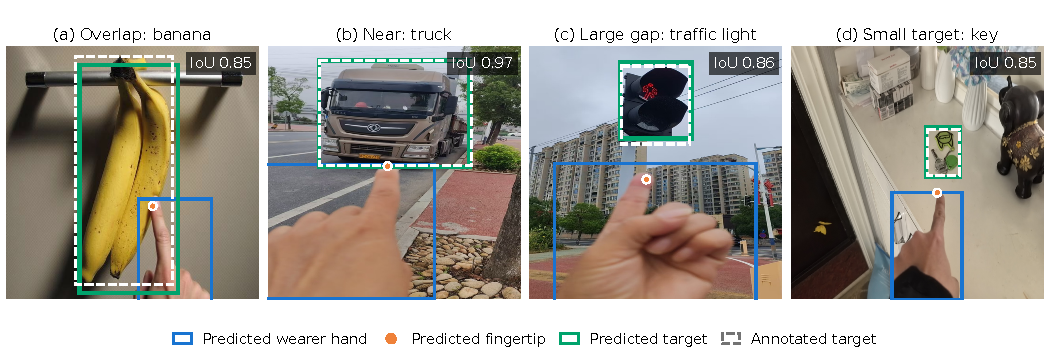
\includegraphics[width=\textwidth]{figures/teaser_successes}
  \caption{SpatialNet's predictions from a single frame: the wearer's hand (blue), the fingertip (orange) and the pointed-at object (green); white dashed: labelled object. The targets overlap the fingertip (a), lie next to it (b), or lie farther away (c, d). Boxes, points and IoUs are the saved predictions of the 160\,px model on EgoPoint test images. These are selected successes, not average accuracy; failures are shown in Figure~\ref{fig:failures}.}
  \Description{Four egocentric photos with predicted boxes that match the labelled boxes: a banana touched by the finger (IoU 0.85), a truck near the fingertip (IoU 0.97), a traffic light far from the fingertip (IoU 0.86), and a small key on a wall (IoU 0.85).}
  \label{fig:teaser}
\end{teaserfigure}

\maketitle

\section{Introduction}\label{sec:intro}

Camera-equipped smart glasses are a fast-growing device category~\cite{idc2026xr,counterpoint2026aiglasses}, and an assistant on them is most useful when the wearer can refer to things in view. Pointing is the most direct way to do so: ``what is \emph{that}?'', ``remind me to buy \emph{this}''. Interfaces have combined speech with pointing since \emph{Put-that-there}~\cite{bolt1980put}, and recent wearable assistants use pointing and gaze to resolve such references~\cite{lee2024gazepointar}. All of them first need the answer to a spatial question, from the glasses' own camera: \emph{which object is the wearer pointing at?}

The models that answer this question best today are large. Multimodal LLMs reason from the hand to a ray and then to the target~\cite{egopoint,li2026pointvgr}, and the most accurate grounding model is a transformer of more than 226M parameters with explicit ray modules~\cite{li2026vistaref}. Such models cannot run on glasses, so every query would send camera frames to a phone or a server. That spends what glasses have least of. Their batteries hold a few hundred milliampere-hours, shared by the camera, audio and radio~\cite{yuan2026aiglasses}; every frame sent adds network latency and server cost; and the frames carry images of bystanders off the device. A model that runs on the glasses avoids all of these costs, provided it is accurate enough to be useful. Existing on-device work stops short of this task: egocentric fingertip systems, one of them on a phone, stop at the fingertip~\cite{huang2016pointing,jain2019gestarlite}, and tiny detectors on smart glasses find generic objects, not the one a gesture refers to~\cite{moosmann2024tinyissimoyolo}. Two difficulties are specific to glasses. The camera sees the wearer's hand from behind and often only in part, and other people's hands can be in view and must not be mistaken for the wearer's.

We therefore ask how much of this task a model small enough for the glasses can do. SpatialNet takes one RGB frame and nothing else: no text prompt, no hand box, no depth, and no external hand detector. In one forward pass of a 0.72M-parameter convolutional network, it predicts the wearer's hand, the fingertip, the pointing direction and the box of the pointed-at object, together with a hand-presence gate. Two design choices address the difficulties above. The prediction heads form a chain in which each head reads a shared feature map at the location that the previous one predicted, so that all outputs belong to the same hand (\emph{instance-anchored heads}). And training pastes other people's hands into the frames without labels and penalises any response to them, so that the model learns to follow the wearer's hand without labelled examples of bystanders.

We evaluate SpatialNet on the EgoPoint benchmark~\cite{egopoint} against published large models and against compact detectors that we train at the same compute and score with the same code, and we deploy it on a pre-production pair of smart glasses. We do not claim a more accurate localiser than large models, or tighter boxes than a compact detector. We show what a sub-million-parameter, image-only model can do on glasses, where it falls short, and which design choices matter at this scale.

\paragraph{Contributions.}
\begin{enumerate}
\item \emph{An image-only pointing-target localiser that runs on smart glasses.} A 0.72M-parameter CNN, at least 300 times smaller than published pointing-grounding models, returns the wearer's hand, fingertip, direction and target box in one pass and runs in 60--80\,ms per frame on a pre-production glasses unit (Sections~\ref{sec:method} and~\ref{sec:ondevice}).
\item \emph{A controlled comparison with compact detectors at the same compute.} Detectors draw tighter boxes, but SpatialNet picks the labelled object more often in every controlled comparison, and an off-the-shelf recogniser names the object from its crops as often as from a detector's (Sections~\ref{sec:comparison} and~\ref{sec:choice}).
\item \emph{Evidence on what matters for small pointing models.} Input resolution is the largest lever for accuracy; instance anchoring makes the hand box and the direction more precise; training with distractor hands keeps accuracy when other people's hands are pasted into the frame, and does so for a generic detector too; and an explicit ray prior is not needed at this scale (Section~\ref{sec:design}). We also find that at least 41\% of the EgoPoint test images are COCO photographs, which benchmarks on this dataset should take into account (Section~\ref{sec:data}).
\end{enumerate}

\section{Related Work}\label{sec:related}

\paragraph{Pointing on wearables.} Deictic gestures have been part of multimodal interfaces since \emph{Put-that-there}~\cite{bolt1980put}, and ray-casting is a standard way to select objects in virtual and augmented reality~\cite{argelaguet2013survey}. Studies of mid-air pointing show systematic offsets~\cite{mayer2015modeling} that accounting for the dominant eye~\cite{plaumann2018towards} and visual feedback such as a cursor~\cite{mayer2018effect} reduce. On smart glasses, the small form factor limits the input options~\cite{lee2018interaction}. GazePointAR resolves spoken pronouns from gaze, pointing and conversation history~\cite{lee2024gazepointar}, and EgoPointVQA answers questions about pointed-at objects by feeding hand keypoints from an off-the-shelf estimator to a multimodal LLM~\cite{choi2026hint}. These systems show the value of pointing on wearables; SpatialNet supplies the localisation step they need, at a cost that fits on the glasses.

\paragraph{Hands, fingertips and pointing targets.} EgoFinger finds the hand and fingertip in egocentric video~\cite{huang2016pointing}, GestARLite runs a fingertip and gesture pipeline on a smartphone~\cite{jain2019gestarlite}, on-device trackers estimate hand keypoints on phones and headsets~\cite{zhang2020mediapipe,han2020megatrack}, and DeePoint estimates the 3D pointing direction from third-person video~\cite{nakamura2023deepoint}; none of them localises the object pointed at. Egocentric hand datasets distinguish the wearer's hands from other people's~\cite{bambach2015lending,shan2020understanding}, but pointing datasets contain only the wearer's hand. YouRefIt grounds targets from language and gesture in third-person views~\cite{chen2021yourefit}. For egocentric images, EgoPoint-Ground introduced the 15K-image benchmark we use and an MLLM baseline that reasons from the hand to a ray and then to the target~\cite{egopoint}. PointVG-R trains this chain of thought into a 7B multimodal LLM with reinforcement learning and names latency as a limitation for wearables~\cite{li2026pointvgr}, and VistaRef adds hand-keypoint and ray modules to a BEiT-3 grounding model and is the most accurate published model on EgoPoint~\cite{li2026vistaref}. General multimodal LLMs still struggle with egocentric pointing~\cite{li2026egopointbench}. Explicit ray reasoning is therefore not new; what differs here is the operating point (Table~\ref{tab:related}).

\paragraph{Efficient models.} Our trunk follows efficient detection design~\cite{ma2018shufflenet,tan2020efficientdet}, and our heads predict keypoint heatmaps in the manner of CenterNet~\cite{zhou2019objects} with a differentiable soft-argmax~\cite{sun2018integral}. Tiny networks run on microcontrollers~\cite{lin2020mcunet} and, for generic object detection, on smart glasses~\cite{moosmann2024tinyissimoyolo}. A compact detector such as YOLO26n~\cite{ultralytics2026yolo26} or NanoDet-Plus~\cite{rangilyu2021nanodet}, trained on pointing data to box the pointed-at object, needs no pointing-specific structure, so we use such detectors as baselines at the same compute. Open-vocabulary detectors and multimodal LLMs ground text queries~\cite{liu2024grounding,peng2023kosmos,you2024ferret,bai2025qwen25vl}, but pointing is not text, and their size rules them out for continuous use on glasses.

\begin{table}[t]
  \caption{Methods that localise pointing or its target. \emph{Hand box}: the ground-truth hand box is an input. Parameter counts as reported; ``$>$1B'': built on a multimodal LLM.}
  \label{tab:related}
  \footnotesize
  \setlength{\tabcolsep}{3pt}
  \begin{tabular}{lllllll}
    \toprule
    Method & View & Test-time input & Output & Params & On device & Other hands \\
    \midrule
    EgoFinger~\cite{huang2016pointing} & ego & image & fingertip & -- & -- & -- \\
    GestARLite~\cite{jain2019gestarlite} & ego & frames & fingertip, gesture & 16.3\,MB & phone & -- \\
    DeePoint~\cite{nakamura2023deepoint} & 3rd & video & pointing, 3D direction & -- & -- & -- \\
    YouRefIt~\cite{chen2021yourefit} & 3rd & image + language & target box & -- & -- & -- \\
    SV-CoT (POG)~\cite{egopoint} & ego & image + hand box & target box & $>$1B & -- & -- \\
    PointVG-R~\cite{li2026pointvgr} & ego & image + instruction & target box & 7B & -- & -- \\
    VistaRef~\cite{li2026vistaref} & ego & image + fixed prompt & target box, keypoints & $\geq$226M & -- & -- \\
    \textbf{SpatialNet} & ego & image & hand, tip, ray, target & 0.72M & glasses & trained \\
    \bottomrule
  \end{tabular}
\end{table}

\section{SpatialNet}\label{sec:method}

\subsection{Task}\label{sec:task}
Given one RGB frame from a head-worn camera, SpatialNet predicts the box $\bH$ of the wearer's hand, the fingertip $\tip$, the pointing direction $\dir$ in the image plane and the box $\bT$ of the pointed-at object, which we call the \emph{target}. It also predicts three presence flags: the wearer's hand is visible, the hand is pointing, and something is pointed at. Boxes and points are normalised to $[0,1]$. Two requirements separate the task from generic detection. \emph{Ownership}: when several hands are visible, all outputs must refer to the wearer's hand, and a frame showing only other people's hands has no wearer's hand. \emph{Budget}: the model must run on the glasses' own processor, without a second network or a server call, within the 100--200\,ms commonly targeted for interactive response~\cite{miller1968response,card1991information}. We do not recognise \emph{what} the target is. $\bT$ is the region that a later step, such as an object recogniser or a visual question-answering model, takes as input, so that this step can run on a small crop and only when the wearer points; Section~\ref{sec:choice} tests such a recogniser.

\subsection{Architecture Overview}\label{sec:arch}
Figure~\ref{fig:arch} shows the network. A shared trunk turns the frame into one feature map $S$. Four heads then run in a fixed order (wearer's hand, fingertip, pointing direction, target), and each head reads $S$ \emph{at the location that the previous head predicted}: the fingertip is searched for around the hand that was found, the direction is computed from features of that hand and fingertip, and the target is searched for along the resulting ray. We call these heads \emph{instance-anchored}. The obvious alternative at this size is to let every head read the same global summary of the frame, a pooled feature vector; nothing then ties the four outputs to one hand, and ablation A4 (Section~\ref{sec:design}) trains that variant for comparison. Three small gates decide which outputs are valid. Everything runs in a single forward pass, with no external hand detector, no language input and no hand box at test time.

\begin{figure}[t]
  \centering
  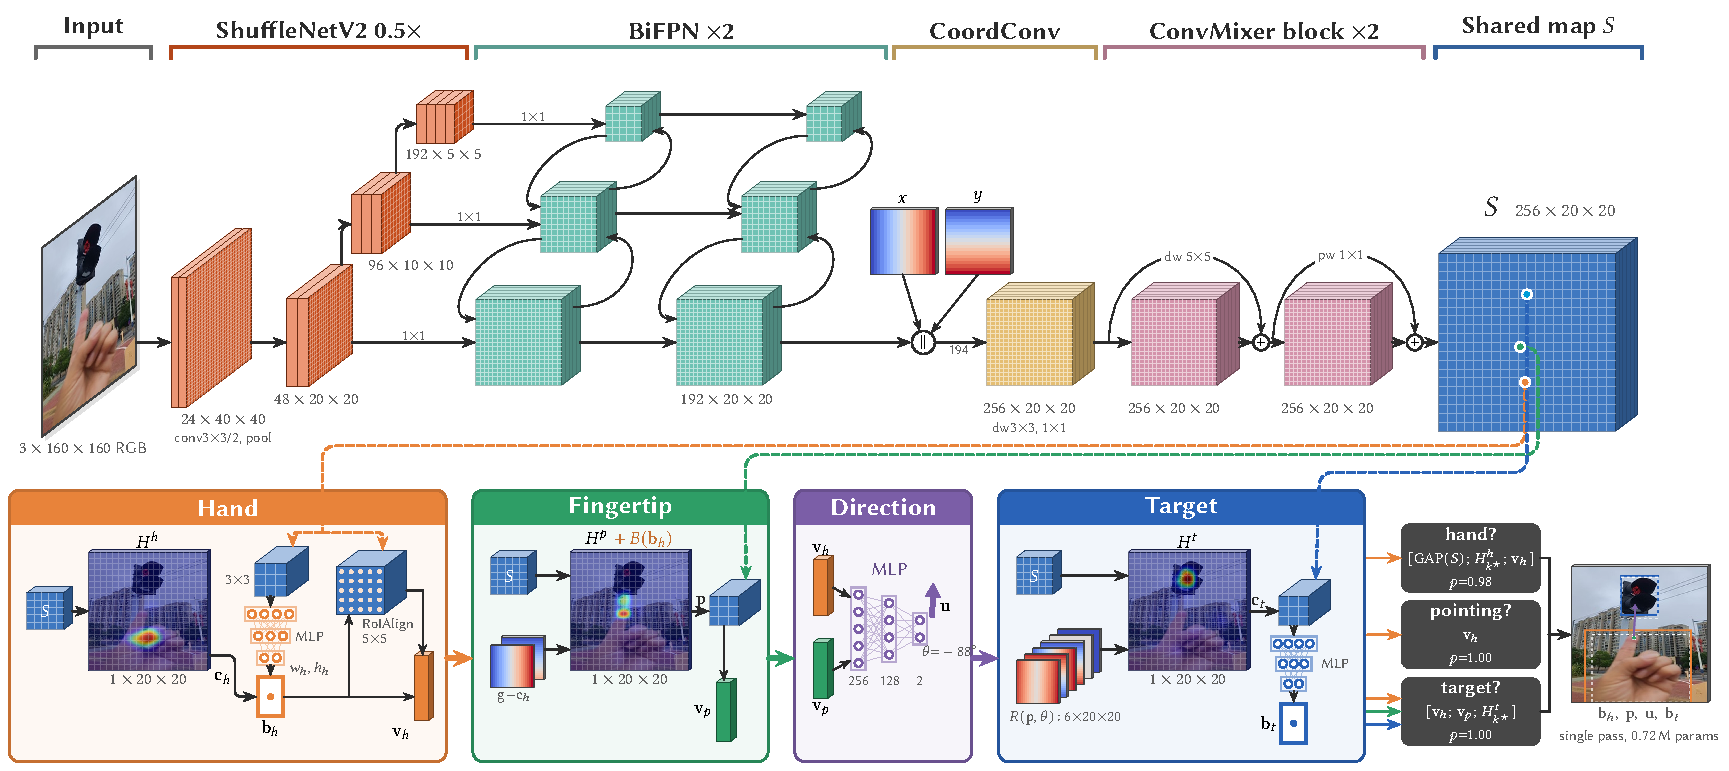
\includegraphics[width=\textwidth]{figures/architecture}
  \caption{SpatialNet. The trunk (top) turns one $160\times160$ frame into the shared map $S$ ($256\times20\times20$). Four heads (middle) run in order; dashed lines mark where a head samples $S$ at the location the previous head predicted: the hand centre $\cH$, the fingertip $\tip$ and the target centre $\cT$. Right: the presence gates and the decoded output. Heatmaps, ray-coordinate maps, gate probabilities and the output are real outputs of the trained model on one test image; each heatmap is overlaid on the input frame.}
  \Description{Block diagram drawn as three-dimensional tensor slabs. The input frame passes through a ShuffleNetV2 backbone whose three scales feed two BiFPN layers; the 20x20 output gets two coordinate channels, is reduced to 256 channels and passes two ConvMixer blocks to give the shared map S. Four coloured panels show the heads in sequence: wearer hand, fingertip, pointing direction and pointed target. Dashed lines from S show where each head samples it. On the right, three presence gates list their inputs and probabilities, and the output frame shows the predicted hand box, fingertip, direction and target box.}
  \label{fig:arch}
\end{figure}

\subsection{Shared Trunk}\label{sec:trunk}
The frame is resized to $160\times160$. A ShuffleNetV2~0.5$\times$ backbone~\cite{ma2018shufflenet} (stages 2--4 only; ImageNet-pretrained~\cite{deng2009imagenet}) gives feature maps at strides 8, 16 and 32, with 48, 96 and 192 channels. Three $1\times1$ convolutions bring all three to 192 channels, and two BiFPN layers~\cite{tan2020efficientdet} merge them into one $192\times20\times20$ map at stride 8. Each fused map is smoothed by a depthwise $3\times3$ convolution with batch normalisation, SiLU, and parameter-free SimAM attention~\cite{yang2021simam}. We then append two coordinate channels (CoordConv~\cite{liu2018coordconv}) and reduce to $D{=}256$ channels with a depthwise-separable convolution. Two ConvMixer-style residual blocks~\cite{trockman2023patches} follow, each made of a depthwise $5\times5$ and a pointwise convolution with residual connections; their batch-norm scales start at zero, so each block is the identity at initialisation. The output is the shared map $S\in\mathbb{R}^{256\times20\times20}$, which all heads read. The $20\times20$ grid places its points about 8 pixels apart at the model input; the heads recover points with sub-cell precision (Section~\ref{sec:softargmax}), so a finer grid would mostly add compute. Sharing one map keeps the heads cheap: the largest head has 104K parameters. The whole network has 722,104 parameters and costs 0.231 GFLOPs per frame, and its FP16 weights take 1.6\,MB (Table~\ref{tab:params}).


\subsection{Locating One Instance: Peak-Windowed Soft-Argmax}\label{sec:softargmax}
Each head predicts a $20\times20$ logit map $H$ and turns it into a point. A global soft-argmax~\cite{sun2018integral} returns the probability-weighted mean over all cells; when two hands are visible, that mean falls \emph{between} them. We therefore restrict the softmax to a $(2r{+}1)\times(2r{+}1)$ window $\mathcal{W}$ around the arg-max cell $k^\star$:
\begin{equation}
\pi_k=\frac{\mathbb{1}[k\in\mathcal{W}]\,\exp(\tau H_k)}{\sum_{j\in\mathcal{W}}\exp(\tau H_j)},\qquad
\hat{\vect{c}}=\sum_k \pi_k\,\cell_k ,
\label{eq:softargmax}
\end{equation}
where $\cell_k\in[0,1]^2$ is the normalised position of cell $k$ and $\tau$ is a temperature; in the implementation the indicator is a large negative offset applied to the logits outside $\mathcal{W}$. The estimate follows a single peak, is differentiable within the window, and is not limited to cell centres. We use $(\tau,r)=(8,2)$ for the hand and the target and $(10,1)$ for the fingertip. The peak logit $H_{k^\star}$ is also passed to the gates as a confidence cue.

\begin{table}[t]
  \caption{Parameters per module. FLOPs are counted by PyTorch's \texttt{FlopCounterMode} (one multiply--accumulate = 2 FLOPs; bilinear sampling not counted) for one $160\times160$ frame. Sizes are serialised state dictionaries.}
  \label{tab:params}
  \small
  \begin{tabular}{lrl}
    \toprule
    Module & Parameters & Role \\
    \midrule
    ShuffleNetV2 0.5$\times$, stages 2--4 & 143,136 & backbone, ImageNet-pretrained \\
    Lateral $1\times1$ projections + BiFPN $\times2$ & 81,426 & multi-scale fusion to stride 8 \\
    CoordConv + reduce & 52,310 & $194\to256$ channels \\
    ConvMixer $\times2$ & 145,920 & context mixing ($5\times5$ depthwise) \\
    \midrule
    Hand head & 104,259 & heatmap, size, descriptor $\vH$ \\
    Fingertip head & 51,826 & incl.\ 12,913 in the hand-offset branch $G^p$ \\
    Direction MLP & 33,154 & $[\vH;\vP]\to\dir$ \\
    Target head & 60,404 & incl.\ 13,105 in the ray branch $G^t$ \\
    Gates (hand / pointing / target) & 24,769 / 8,321 / 16,577 & presence logits \\
    Learnable scales $\alpha_p,\alpha_t$ & 2 & \\
    \midrule
    \textbf{Total} & \textbf{722,104} & 0.231 GFLOPs; 3.0\,MB FP32; 1.6\,MB FP16 \\
    \bottomrule
  \end{tabular}
\end{table}

\subsection{Instance-Anchored Heads}\label{sec:heads}

\paragraph{Wearer's hand.} A depthwise $3\times3$ and pointwise head gives hand-centre logits $H^h$, and Eq.~\eqref{eq:softargmax} gives the centre $\cH$. For the box size $(w_h,h_h)$, we sample a $3\times3$ neighbourhood of $S$ around $\cH$ bilinearly (one-cell spacing). A depthwise $3\times3$ convolution and a pointwise projection collapse it to 128 dimensions, and a two-layer MLP with a sigmoid maps it to the size, giving $\bH=(\cH,w_h,h_h)$. To describe \emph{this} hand instance, we sample a $5\times5$ RoIAlign-style lattice~\cite{he2017mask} over $\bH$ enlarged by 1.15, collapse it to 128 dimensions, and fuse it with the box coordinates into the hand descriptor $\vH\in\mathbb{R}^{128}$.

\paragraph{Fingertip.} The fingertip must belong to the hand just found. Its logits add three terms:
\begin{equation}
H^p = V^p(S) + G^p\big([S;\,\alpha_p(\cell-\cH)]\big) + B(\bH).
\label{eq:tip}
\end{equation}
$V^p$ is a visual head of the same form as the hand head. $\alpha_p(\cell-\cH)$ are two channels holding each cell's offset to the hand centre, with a learnable scale $\alpha_p$, and $G^p$ is a small branch (a $1\times1$ convolution to 48 channels, then a $3\times3$ convolution to one channel, with its last layer initialised at zero) that learns where fingertips lie relative to the hand centre. $B$ is a fixed log-prior that is zero inside the hand box dilated by $\delta{=}1.3$ and falls linearly outside it:
\begin{equation}
B_k(\bH) = -\frac{\lambda}{\tau_p}\Big(\big[\tfrac{|g_{k,x}-c_{h,x}|}{\delta w_h/2}-1\big]_+ + \big[\tfrac{|g_{k,y}-c_{h,y}|}{\delta h_h/2}-1\big]_+\Big),
\label{eq:boxprior}
\end{equation}
where $[\cdot]_+=\max(\cdot,0)$ and each half-width in the denominator is clamped to at least one cell. With $\lambda{=}4$, the penalty after the softmax temperature $\tau_p$ is 4 logits for every half box-width outside the dilated box, and no gradient flows from the prior into $\bH$. In the training labels, the fingertip lies inside the dilated box in 99.4\% of pointing images, so the prior rarely contradicts a label while it rules out the fingertips of other hands. Eq.~\eqref{eq:softargmax} (with $r{=}1$) gives the fingertip $\tip$, and a $3\times3$ sample around it gives the fingertip descriptor $\vP\in\mathbb{R}^{128}$.

\paragraph{Pointing direction.} An MLP ($256\to128\to2$, $\tanh$) maps $[\vH;\vP]$ to a vector, which we L2-normalise into the unit direction $\dir=(\cos\theta,\sin\theta)$ in image coordinates. The direction is supervised with the image-plane direction from the labelled fingertip to the labelled target centre (Section~\ref{sec:losses}), so $\dir$ is the direction \emph{to the target} as it appears in the image, not the 3D orientation of the finger.

\paragraph{Pointed target.} The target head is given the geometry of the predicted ray explicitly. From $\tip$ and $\dir$, every cell $k$ receives six \emph{ray coordinates}:
\begin{equation}
\Delta_k=\alpha_t(\cell_k-\tip),\qquad
t_k=\Delta_k\cdot\dir,\qquad
s_k=\big|\Delta_{k,x}\sin\theta-\Delta_{k,y}\cos\theta\big|,\qquad
\cos\theta,\qquad \sin\theta .
\label{eq:raycoords}
\end{equation}
These are the scaled offset from the fingertip (two channels), the signed distance along the ray (negative behind the fingertip), the distance from the line of the ray, and the direction itself. The target logits are
\begin{equation}
H^t = V^t(S) + G^t\big([S;\,R(\tip,\theta)]\big),
\label{eq:target}
\end{equation}
where $R$ stacks the six maps, and $G^t$ (13K parameters) has the form of $G^p$ and also starts at zero. The soft-argmax applies a softmax to $\tau H^t$, so $\pi_k\propto\exp(\tau V^t_k)\exp(\tau G^t_k)$: although the two terms are added in logit space, the geometry term acts as a learned \emph{multiplicative prior} on the visual evidence. Because $G^t$ starts at zero, training begins with a purely visual head, and the network uses the ray only as far as it lowers the loss. We let the network learn the shape of this prior, instead of fixing a cone, because the right shape depends on the gap: when the fingertip overlaps the target (about 70\% of EgoPoint targets, Section~\ref{sec:data}), the target centre can lie in any direction from the fingertip, while for targets far from the fingertip a narrow band along the ray is informative. Whether the network exploits this freedom is an empirical question; Section~\ref{sec:design} shows that on EgoPoint it learns mainly a fingertip-proximity prior. The target centre $\cT$ follows from Eq.~\eqref{eq:softargmax}, and its size comes from a $3\times3$ sample, as for the hand, giving $\bT=(\cT,w_t,h_t)$.

\subsection{Presence Gates and Scene Decoding}\label{sec:gates}
Three MLP gates output logits for whether the wearer's hand is present (from $[\mathrm{GAP}(S);\,H^h_{k^\star};\,\vH]$), whether it is pointing (from $\vH$ alone) and whether something is pointed at (from $[\vH;\vP;H^t_{k^\star}]$). At inference they form a cascade with threshold 0.5: if the hand gate is off, the frame is \emph{no hand}; otherwise the pointing gate and then the target gate decide between \emph{hand, not pointing}, \emph{pointing, no target} and \emph{pointing at a target}. The pointing and target gates read instance descriptors rather than the whole image, so that another person's pointing hand elsewhere in the frame is not meant to switch them on by itself. The hand gate also sees the global pool, so that a frame containing only other people's hands can be classed as having \emph{no wearer's hand}. EgoPoint contains only the first and last of these four scenes (Section~\ref{sec:data}), so we evaluate the hand gate and make no claims about the pointing and target gates.

\subsection{Learning Whose Hand It Is}\label{sec:ownership}
No public pointing dataset labels other people's hands, and EgoPoint frames contain only the wearer's. We therefore paste hands into the frames during training (Figure~\ref{fig:ownership}). The procedure follows copy-paste augmentation~\cite{dwibedi2017cut,ghiasi2021simple}, but with the opposite aim: pasted hands are \emph{not} labelled, and the model is penalised for responding to them. One or two hand crops from other training images are pasted into half of the images with a hand and 30\% of those without, mostly rotated and placed in the upper part of the frame, away from the wearer's hand and the target. In 30\% of cases the pasted crop is the wearer's own hand, so that appearance alone cannot tell the two apart and the model has to use position, orientation and context. Labels never change: a no-hand image with a pasted hand stays \emph{no hand}, which teaches the hand gate to answer for the wearer only. In the hand-heatmap loss, the negative term near a pasted hand is multiplied by $1+4\,G_k$, where $G_k$ is a Gaussian ($\sigma{=}1.5$ cells) at that hand's centre, so that a response on another person's hand costs up to five times as much as one on background. Appendix~\ref{app:aug} lists all settings.

\emph{The prior this encodes.} The procedure assumes that, from a head-worn camera, the wearer's arm enters from the bottom of the frame, while other people's hands appear higher and in other orientations. This holds for most use of glasses but not always, for example when the wearer raises a hand above eye level or when a companion's hand is near the bottom of the view (Section~\ref{sec:discussion}).

\begin{figure}[t]
  \centering
  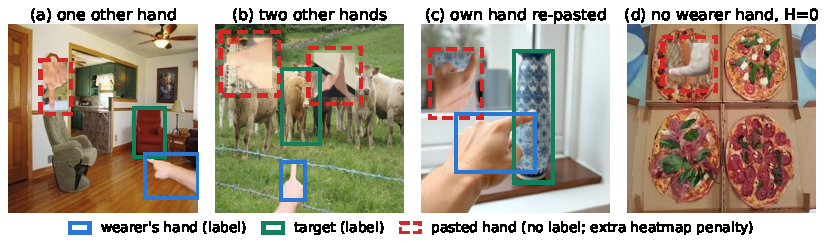
\includegraphics[width=\linewidth]{figures/ownership_examples}
  \caption{Distractor-hand pasting, produced by the training code. Pasted hands (red, dashed) come from other images (a, b) or from the same image (c), are rotated so that they rarely enter from the bottom edge, and are never labelled. A no-hand image with a pasted hand keeps the label \emph{no hand} (d).}
  \Description{Four training images. In the first two, one or two hands cut from other photos are pasted into the upper part of the image, rotated, and marked with red dashed boxes, while the wearer's pointing hand and the target keep their blue and green label boxes. In the third, a rotated copy of the wearer's own hand is pasted in the upper left. In the fourth, a pizza photo without a wearer's hand receives a pasted hand and keeps the label no hand.}
  \label{fig:ownership}
\end{figure}

\subsection{Training Objective}\label{sec:losses}
The loss is a weighted sum of 13 terms (Table~\ref{tab:weights}), each computed only on images whose label contains the parts it needs. \emph{Localisation} uses the CIoU loss for the hand box~\cite{zheng2020distance}; the Wing loss~\cite{feng2018wing} for the fingertip, on normalised coordinates with $w{=}0.5$ and $\epsilon{=}0.1$; $1-\cos(\dir,\dir^\star)$ for the direction, where $\dir^\star$ is the unit vector from the labelled fingertip to the labelled target centre; and the SIoU loss~\cite{gevorgyan2022siou} plus $1-\mathrm{IoU}$ for the target box. \emph{Heatmaps} use the penalty-reduced focal loss of CornerNet and CenterNet~\cite{law2018cornernet,zhou2019objects} ($\alpha{=}2$, $\beta{=}4$) on Gaussian targets at the hand centre, fingertip and target centre ($\sigma$ = 1.5, 0.8 and 1.2 cells), which gives each heatmap a direct signal in addition to the gradient through the soft-argmax. \emph{Gates} use focal binary cross-entropy~\cite{lin2017focal} ($\gamma{=}2$), each on its own population (the hand gate on all images, the pointing gate on hand images, the target gate on pointing images), with positives weighted $2\times$ ($3\times$ for the hand gate), because a missed pointing gesture costs the user more than a false alarm that the interface can ignore.

\emph{Geometric consistency} adds two terms that use predictions only. The ray-alignment term asks the predicted target centre to lie on the predicted ray, in front of the fingertip:
\begin{equation}
\mathcal{L}_{\mathrm{ray}} = \big\|\vect{r}-(\vect{r}\cdot\hat{\dir})\,\hat{\dir}\big\| + 0.5\,\big[-\vect{r}\cdot\hat{\dir}\big]_+,\qquad \vect{r}=\hat{\vect{c}}_t-\hat{\tip}.
\label{eq:rayloss}
\end{equation}
Because $\dir^\star$ runs from the labelled fingertip to the labelled target centre, the ground truth gives $\mathcal{L}_{\mathrm{ray}}=0$ exactly: the term does not move the optimum and only penalises predictions that disagree with each other. For a fixed angular error, it grows with the fingertip--target distance, so it weighs targets far from the fingertip most. The hand-axis term is a hinge that keeps $\hat{\dir}$ within $60^\circ$ of the axis from the predicted hand centre to the predicted fingertip. It is only a weak plausibility prior, since the labelled direction lies inside this cone in 68.6\% of training images, so it has the smallest weight of all 13 terms. The weights were set by hand during development, using the training and validation splits only, and were not tuned by a search; ablation A2 (Section~\ref{sec:design}) removes the two consistency terms.

\begin{table}[t]
  \caption{Loss terms, their supervision, and weights.}
  \label{tab:weights}
  \footnotesize
  \begin{tabular}{llll}
    \toprule
    Term & Loss & Supervision & Weight \\
    \midrule
    Hand box & 1 $-$ CIoU & hand box & 0.10 \\
    Fingertip & Wing ($w{=}0.5$, $\epsilon{=}0.1$) & fingertip & 0.18 \\
    Direction & 1 $-$ cosine & fingertip $\to$ target centre & 0.03 \\
    Target box & 1 $-$ SIoU & target box & 0.45 \\
    Target box, auxiliary & 1 $-$ IoU & target box & 0.10 \\
    Hand gate & focal BCE, positives $\times3$ & $H$ & 0.08 \\
    Pointing gate & focal BCE, positives $\times2$ & $P$ (hand images) & 0.10 \\
    Target gate & focal BCE, positives $\times2$ & $T$ (pointing images) & 0.06 \\
    Ray alignment & distance to ray $+$ 0.5 $\cdot$ behind & none (predictions only) & 0.08 \\
    Hand axis & hinge outside a $60^\circ$ cone & none (predictions only) & 0.02 \\
    Hand heatmap & penalty-reduced focal, ownership-weighted & hand centre & 0.10 \\
    Fingertip heatmap & penalty-reduced focal & fingertip & 0.10 \\
    Target heatmap & penalty-reduced focal & target centre & 0.10 \\
    \bottomrule
  \end{tabular}
\end{table}

\subsection{Scheduled Anchor Forcing}\label{sec:forcing}
Early in training, the predicted hand centre, fingertip and target centre are close to random, so the downstream heads would read features at meaningless locations. As in scheduled sampling for sequence models~\cite{bengio2015scheduled}, we sometimes replace each anchor with its ground-truth location, independently per image and per anchor, with a probability that decreases linearly from 0.5 to 0 over the first 20 epochs. From then on, training uses the model's own anchors, as at test time. Appendix~\ref{app:method} gives the training schedule and the augmentation settings.

\section{Experimental Setup}\label{sec:setup}

\subsection{Data}\label{sec:data}
We train and test on the image set of EgoPoint-Ground~\cite{egopoint}, which we call EgoPoint, with its official split. Its paper reports that 39\% of the images are real captures with smart glasses and the rest are synthetically composed or edited; the release does not mark which is which, so, like other work on this benchmark~\cite{li2026vistaref,li2026pointvgr}, we report on the whole test split. After converting the labels (Appendix~\ref{app:data}), the test split has 2,604 images of the wearer pointing at a target and 425 images without a hand. We dropped 43 test images whose fingertip is not annotated, which changes the reported accuracy by less than one point. EgoPoint has no frames with a non-pointing hand and none with pointing but no target, so we evaluate the hand gate but not the pointing and target gates. In about 70\% of the images, the fingertip lies inside the target box.

\paragraph{COCO overlap.} The edited images were made by adding a pointing hand to photographs from COCO~\cite{lin2014coco}, selected through RefCOCO~\cite{yu2016modeling}, and the release names each source photograph. At least 41\% of our test images (1,242 of 3,029) are COCO train2014 photographs, which every COCO-pretrained detector has seen in training, together with box labels for the objects they contain. We therefore separate COCO-pretrained baselines from those that, like SpatialNet, never saw COCO data, and test whether the overlap inflates their scores (Section~\ref{sec:comparison}).

\subsection{Metrics}\label{sec:metrics}
The main metric is \emph{P@0.5}, the share of test images whose predicted target box overlaps the labelled box with IoU${\geq}0.5$, the standard grounding metric on this benchmark~\cite{egopoint,li2026vistaref,li2026pointvgr}; P@0.7 and the mean IoU (mIoU) measure how tight the boxes are. \emph{Centre in target}, the share of images whose predicted target centre lies inside the labelled box, measures whether the model picked the right object, independently of how well it drew the box. In a \emph{recognition test}, an off-the-shelf zero-shot recogniser chooses among the 348 target category names of EgoPoint from a crop of each model's predicted box, as a ``what is that?'' assistant would. We use two recognisers trained with different objectives, CLIP ViT-B/16~\cite{radford2021clip} and SigLIP base~\cite{zhai2023siglip}, without any training, and a crop counts as recognised if the top-ranked name is the labelled category (Appendix~\ref{app:recog}). Differences between models are tested with paired bootstrap intervals over the test images (1,000 resamples). For ablations, a difference counts as an effect only if its interval excludes zero \emph{and} it exceeds the change that retraining the full model with another seed produces.

\subsection{Baselines}\label{sec:baselines}
\paragraph{Published large models.} We copy the reported results of VistaRef~\cite{li2026vistaref}, PointVG-R and the multimodal LLMs that it evaluates~\cite{li2026pointvgr}. We did not re-run them, and their protocols differ slightly from ours (Appendix~\ref{app:comparison}), so we read differences from them as large gaps, not precise ones.

\paragraph{Compact detectors at the same compute.} YOLO26n~\cite{ultralytics2026yolo26} at a 128\,px input (0.225 GFLOPs) and NanoDet-Plus-m~\cite{rangilyu2021nanodet} at 160\,px (0.218 GFLOPs) cost about as much compute as SpatialNet (0.231 GFLOPs). Each is trained on the same split to output one box for the wearer's hand and one for the target, and is scored by the same code on the same images. Besides a benchmark of both detectors from several starting points (Appendix~\ref{app:comparison}), we trained YOLO26n four times under one fully specified recipe: from ImageNet weights, the pretraining of our own backbone, with two seeds; from ImageNet weights with our distractor pasting; and from COCO weights.

\subsection{Implementation and Deployment}\label{sec:device}
We train with AdamW and a one-cycle schedule for up to 180 epochs, with early stopping on the validation loss, on one NVIDIA T4 (1\,h\,40\,min, seed 42); Appendix~\ref{app:method} lists all settings. Retraining with seeds 1 and 2 gives the same target P@0.5 (58.9--59.0\% in all three runs), and the spread across seeds calibrates the single-run comparisons below.

We deploy the 160\,px model, exported to ONNX and FP16, on an engineering unit of a pair of smart glasses: a pre-production test device, not a retail product. It has a smart-glasses system-on-chip with a low-power microcontroller, a 12\,MP ultra-wide camera in portrait orientation, a wireless link to a companion phone and a 160\,mAh battery. The model squashes the portrait frames to its square input, as it does with the mostly landscape training images. Because the unit's power management is not tuned for production, we treat it as a measurement platform and compare two operating modes on the same unit rather than report battery life: \emph{on the glasses}, SpatialNet runs continuously on camera frames; in \emph{offloading}, the glasses only capture frames and send them to the phone at 0.5 frames per second, where localisation would run on the phone or in the cloud.

\section{Results}\label{sec:results}

\subsection{Comparison with Large Models and Compact Detectors}\label{sec:comparison}

SpatialNet finds the wearer's hand reliably: its hand box reaches IoU${\geq}0.5$ in 92.6\% of test images, and its fingertip error is 3.9\,px at the $160\times160$ input (Appendix~\ref{app:heads}). The harder part is the target. Table~\ref{tab:main} places SpatialNet between two reference points.

\begin{table}[t]
  \caption{Target localisation on the EgoPoint test split (\%). Published results are copied, not re-run, and their protocols differ slightly from ours (Appendix~\ref{app:comparison}). The compact detectors were trained on the same split and scored by the same code as SpatialNet; the YOLO26n rows are our controlled runs (seed 42), and NanoDet-Plus-m comes from our benchmark. \emph{Centre in}: predicted target centre inside the labelled box. $^\dagger$\,Pretrained on COCO, the source of at least 41\% of the test images.}
  \label{tab:main}
  \footnotesize
  \setlength{\tabcolsep}{3.5pt}
  \begin{tabular}{lrrrrrr}
    \toprule
    Method & Params & GFLOPs & P@0.5 & P@0.7 & mIoU & Centre in \\
    \midrule
    \multicolumn{7}{l}{\emph{Large models trained on EgoPoint (published)}} \\
    \quad VistaRef, BEiT-3-L & $>$226M & -- & 93.9 & 82.6 & 82.0 & -- \\
    \quad PointVG-R, Qwen2.5-VL-7B, SFT + RL & 7B & -- & 83.6 & 74.5 & 75.7 & -- \\
    \quad Qwen2.5-VL-7B, SFT & 7B & -- & 63.6 & 56.7 & 59.8 & -- \\
    \multicolumn{7}{l}{\emph{Multimodal LLM without training on EgoPoint (published)}} \\
    \quad Qwen2.5-VL-7B, zero-shot & 7B & -- & 49.8 & 42.9 & 45.5 & -- \\
    \multicolumn{7}{l}{\emph{Compact detectors at the same compute (trained by us)}} \\
    \quad YOLO26n, 128\,px, ImageNet start & 2.50M & 0.225 & 62.9 & 43.4 & 56.4 & 82.1 \\
    \quad YOLO26n, 128\,px, COCO start$^\dagger$ & 2.50M & 0.225 & 64.4 & 45.5 & 58.3 & 82.2 \\
    \quad NanoDet-Plus-m, 160\,px, COCO start$^\dagger$ & 1.17M & 0.218 & 67.6 & 49.5 & 59.8 & 82.9 \\
    \midrule
    \textbf{SpatialNet}, 160\,px (deployed) & \textbf{0.72M} & 0.231 & 58.9 & 31.8 & 53.3 & \textbf{84.8} \\
    \quad same model, 320\,px input & 0.72M & 0.923 & 65.1 & 40.3 & 56.5 & -- \\
    \bottomrule
  \end{tabular}
\end{table}

\paragraph{Large models are far more accurate.} VistaRef places a correct box on the target in 94\% of test images, against 59\% for SpatialNet, and its boxes are much tighter. These models are 300 to 10{,}000 times larger and run on GPUs; SpatialNet gives up this accuracy for a model that runs on the glasses. Against a 7B multimodal LLM used without training on EgoPoint, SpatialNet finds the target more often (P@0.5 of 59 against 50\%) but draws looser boxes; given the protocol differences, we read this as the same accuracy range at a fraction of the size, not as superiority. The target head does real work: a box of mean size placed at the labelled fingertip reaches a P@0.5 of only 11\%, because target sizes vary widely (Appendix~\ref{app:comparison}).

\paragraph{At the same compute, compact detectors draw tighter boxes.} With the same ImageNet pretraining as our backbone, YOLO26n is 4.0 points higher in P@0.5 (95\% paired interval [2.2, 6.0]) and 11.6 points higher in P@0.7, and a second training seed gives the same picture. The COCO-pretrained detectors score higher still. The COCO overlap does not explain their lead: against the ImageNet start, the COCO start gains 2.4 points [0.6, 4.3] on the test images that do not come from COCO and nothing on those that do (Appendix~\ref{app:coco}), so its advantage is general transfer, not recall of the test photographs. Resolution narrows the gap, but only at a cost: SpatialNet at 320\,px reaches 65.1\% with four times the compute, where compact detectors improve too (COCO-pretrained YOLO26n at 192\,px reaches 69.9\% with 0.51 GFLOPs; Appendix~\ref{app:comparison}).

\subsection{Target Choice and Downstream Recognition}\label{sec:choice}

\paragraph{SpatialNet picks the labelled object more often.} Its predicted target centre lies inside the labelled box in 84.8\% of test images, against 81.6--82.2\% for the four controlled detectors, and every paired difference (2.6 to 3.2 points) has an interval that excludes zero. SpatialNet's deficit therefore lies in how far the object extends, not in which object it picks: in 26\% of the test images its box misses IoU 0.5 although its centre lies on the labelled object.

\paragraph{A recogniser names the object from its crops as often as from a detector's.} A ``what is that?'' assistant does not need a tight box; it needs the object's name. Table~\ref{tab:recog} shows how often each recogniser names the labelled category from a crop of each model's box. With both recognisers, SpatialNet's crops are named correctly as often as the detectors' crops: the paired differences lie between $-$1.3 and $+$0.3 points, and every interval includes zero and lies within $\pm$2.8 points. Localisation matters, since SpatialNet's crops are named correctly 6--8 points more often than the whole frame and reach about 90\% of the rate for crops of the labelled box. Its loose but well-centred boxes explain the result: they are still named correctly in 47--51\% of cases, close to the 54--58\% for boxes with IoU${\geq}0.5$. The exception is targets far from the fingertip, where the detectors' crops are named 4--8 points more often, in line with their better boxes there (Appendix~\ref{app:recog}).

\begin{table}[t]
  \caption{Downstream recognition: how often an off-the-shelf zero-shot recogniser names the labelled category from a crop of each model's target box, choosing among the 348 EgoPoint category names (top-1 accuracy, \%, on the 2,603 test targets with a category name). The labelled box and the whole frame are references. A box on a neighbouring object of the same category counts as correct.}
  \label{tab:recog}
  \footnotesize
  \begin{tabular}{lrr}
    \toprule
    Crop & CLIP ViT-B/16 & SigLIP base \\
    \midrule
    Labelled box (upper reference) & 53.9 & 59.4 \\
    Whole frame (lower reference) & 40.3 & 46.2 \\
    \midrule
    \textbf{SpatialNet} & 48.6 & 52.3 \\
    YOLO26n, ImageNet start (seeds 42 / 1) & 48.8 / 49.1 & 53.3 / 53.4 \\
    YOLO26n, ImageNet start + pasting & 49.9 & 52.0 \\
    YOLO26n, COCO start & 49.1 & 53.2 \\
    \bottomrule
  \end{tabular}
\end{table}

\paragraph{What this means.} For an application that needs a tight box, a compact detector is the better choice at this compute. For naming the target, SpatialNet does as well, and it also returns the hand, the fingertip and the direction from the same pass, with fewer parameters (0.72M, against 1.17M for NanoDet-Plus-m and 2.50M for YOLO26n). An interface can use these outputs for feedback, such as a fingertip cursor or the pointing ray, which helps mid-air pointing~\cite{mayer2018effect}, and for gating on hand presence. Whether users benefit from them, we did not test.

\subsection{What Matters at This Scale}\label{sec:design}

\paragraph{Input resolution is the largest lever.} Retraining the unchanged model at 224 and 320\,px raises P@0.5 from 58.9\% to 62.4\% and 65.1\%, a gain of 6.2 points at 320\,px (interval [4.4, 8.0]) at no parameter cost, against a spread of 0.1 points between seeds. A larger backbone does not help in the same way: MobileNetV3-Small and MobileNetV4-Conv-Small double or nearly triple the parameters without a significant change in P@0.5 (Appendix~\ref{app:backbone}). Extra compute is therefore best spent on the input. It costs two and four times the compute of the deployed model, which we have not yet measured on the glasses.

\paragraph{What each component adds.} Table~\ref{tab:ablation} retrains the 160\,px model without one component at a time. No component changes P@0.5 by more than 1.1 points; each adds a specific capability, at a cost of at most 13K parameters.
\begin{itemize}
\item \emph{Instance anchoring} (A4) makes the hand box and the direction more precise. Against a plain model of the same size, whose heads read a globally pooled feature, it improves the hand mIoU by 1.8 points [1.4, 2.2] and lowers the direction error by 3.4$^\circ$ [2.4, 4.5], both beyond the change from retraining.
\item \emph{Distractor pasting} (A1) keeps accuracy when other hands are in view. With one or two hands pasted into each test image, the model trained with pasting keeps 4.1 more points of P@0.5 [2.4, 5.8] and classifies 5.4 more points of no-hand frames correctly [1.9, 8.9], at no cost on clean images. The recipe is not specific to SpatialNet: YOLO26n trained with the same pasting becomes as stable as SpatialNet, whereas detectors trained without it lose 2.4--4.6 points of P@0.5 under pasted hands (Appendix~\ref{app:controlled}). Both tests use pasted hands, which resemble the training distribution; real bystander hands remain untested.
\item \emph{Explicit ray geometry} (A3) is not needed at this scale: removing the ray branch does not lower accuracy. Probing the trained model shows why. The branch has learned mainly that targets lie near the fingertip, which fits the 70\% of targets that the fingertip overlaps, rather than where the ray points, and neither restricting it to the space in front of the fingertip nor up-weighting targets away from the fingertip changes this (Appendix~\ref{app:ray}). We keep the branch in the deployed model because that is the model measured on the glasses.
\item The two \emph{consistency losses} (A2) sharpen the direction, not the box.
\end{itemize}

\begin{table}[t]
  \caption{Ablations at 160\,px (one training run each). First row: the full model; other rows: difference from it (points; degrees for the direction error, where positive means worse). \emph{Retraining}: the largest change that retraining the full model with seeds 1 and 2 produced. Bold: the 95\% paired interval excludes 0 and the difference exceeds the retraining row. $^\S$\,Not significant once duplicated test images are removed. \emph{With other hands}: one or two hands pasted into each test image. All columns are in Appendix~\ref{app:ablation}.}
  \label{tab:ablation}
  \footnotesize
  \setlength{\tabcolsep}{4pt}
  \begin{tabular}{lrrrrrr}
    \toprule
    & \multicolumn{4}{c}{Clean test images} & \multicolumn{2}{c}{With other hands} \\
    \cmidrule(lr){2-5}\cmidrule(l){6-7}
    Variant & P@0.5 & P@0.7 & Hand mIoU & Direction ($^\circ$) & P@0.5 & No hand kept \\
    \midrule
    Full model & 58.9 & 31.8 & 73.7 & 32.2 & 60.1 & 91.8 \\
    \quad Retraining (seeds 1, 2) & $\pm$0.1 & $\pm$0.8 & $\pm$0.3 & $\pm$1.2 & $\pm$0.4 & $\pm$3.3 \\
    \midrule
    A1 no distractor pasting & $-$0.1 & $-$1.3 & \textbf{$-$0.6} & \textbf{$+$1.8} & \textbf{$-$4.1} & \textbf{$-$5.4} \\
    A2 no consistency losses & $+$1.1 & $+$0.6 & $-$0.4 & \textbf{$+$1.5} & 0.0 & $-$1.2 \\
    A3 no ray branch & $+$0.7 & \textbf{$+$1.9}$^\S$ & 0.0 & \textbf{$-$1.3} & $+$1.0 & $+$1.2 \\
    A4 no instance anchoring & $-$0.3 & \textbf{$-$2.8}$^\S$ & \textbf{$-$1.8} & \textbf{$+$3.4} & $-$0.5 & 0.0 \\
    \bottomrule
  \end{tabular}
\end{table}

\subsection{On the Glasses}\label{sec:ondevice}

\begin{table}[t]
  \caption{Cost of the 160\,px model on the engineering unit of Section~\ref{sec:device}, with a server CPU for reference. The battery rows are single one-minute observations. $^\ast$\,Derived from the per-frame latency, assuming frames are processed back to back.}
  \label{tab:device}
  \footnotesize
  \begin{tabular}{lr}
    \toprule
    Measure & Value \\
    \midrule
    Glasses: inference latency per frame & 60--80\,ms \\
    Glasses: throughput$^\ast$ & 12--17 frames/s \\
    Glasses: peak additional RAM during inference & ${\approx}$100\,KB \\
    Glasses: battery drain in one minute, SpatialNet running continuously & 9\% \\
    Glasses: battery drain in one minute, streaming frames to the phone at 0.5\,fps & 16\% \\
    \midrule
    Server CPU (1 thread), PyTorch: latency, median & 25.7\,ms \\
    \bottomrule
  \end{tabular}
\end{table}

SpatialNet takes 60--80\,ms per frame on the glasses (Table~\ref{tab:device}), within the 100--200\,ms targeted for interactive response~\cite{miller1968response,card1991information}, and needs about 100\,KB of RAM beyond the idle application, with 1.6\,MB of FP16 weights. Running the weights in half precision gives the same target IoU as full precision on 320 validation images, so halving the model size costs no accuracy. Over one minute, continuous inference used 9 percentage points of charge, and streaming frames to the phone at 0.5\,fps used 16, although streaming sends one frame every two seconds while SpatialNet processes frames continuously. Each mode was measured once on an engineering unit without production power management, so this indicates the relative cost of the two modes on this unit only; it is not an energy measurement or a battery-life estimate. Continuous inference is the worst case: in use, the model would run only while the wearer points.

\subsection{Frames from the Glasses' Camera}\label{sec:realframes}

All accuracy figures above come from EgoPoint, whose images are mostly landscape and partly composed or edited. As a check of transfer to the deployed camera, \tbd{K} wearers recorded \tbd{N} frames with the glasses while pointing at everyday objects at different distances in \tbd{places}, and \tbd{M} frames with no hand in view. For each pointing frame, the wearer named the object they meant; afterwards, \tbd{two annotators} drew the boxes of that object and of the wearer's hand without seeing the model's outputs. We score the outputs that the model produced on the glasses with the metrics of Section~\ref{sec:metrics} and give Wilson intervals (Table~\ref{tab:real}); Figure~\ref{fig:real} shows examples. \tbd{One or two sentences on the result: whether the hand, the target and the centre in target stay close to the EgoPoint values, and which failure types of Section~\ref{sec:failures} appear.} With \tbd{N} frames, this check can reveal a large drop in accuracy but not a small one.

\begin{table}[t]
  \caption{The deployed model on EgoPoint and on frames from the glasses' camera, scored with the same metrics (\%; brackets: 95\% Wilson intervals). \emph{No hand kept}: frames without a hand classed as no hand, at the hand-gate threshold of 0.5.}
  \label{tab:real}
  \footnotesize
  \begin{tabular}{lrrrrr}
    \toprule
    Frames & Pointing / no hand & Hand P@0.5 & Target P@0.5 & Centre in & No hand kept \\
    \midrule
    EgoPoint test split & 2,604 / 425 & 92.6 & 58.9 & 84.8 & 93.4 \\
    Glasses' camera & \tbd{N} / \tbd{M} & \xx\ [\xx, \xx] & \xx\ [\xx, \xx] & \xx\ [\xx, \xx] & \xx\ [\xx, \xx] \\
    \bottomrule
  \end{tabular}
\end{table}

\begin{figure}[t]
  \centering
  \phfig{\linewidth}{3.2cm}{Six frames from the glasses' camera with SpatialNet's on-device outputs (hand, fingertip, ray, target) and the annotated target. Include at least one failure.}
  \caption{Frames from the glasses' camera. \tbd{Insert after the real-frame check.}}
  \Description{To be inserted: six photos from the glasses showing SpatialNet's outputs and the annotated target.}
  \label{fig:real}
\end{figure}

\subsection{Where SpatialNet Fails}\label{sec:failures}

We sorted the 558 test images with a target IoU below 0.3 by rule. In 36\% of them, the model found the right object but drew the wrong extent, for example part of a bed instead of the whole bed. In 33\%, the direction was wrong, and in 31\%, the model chose a neighbouring object despite a reasonable direction, typically a similar object next to the labelled one. The hand was missed in 1\%. Figure~\ref{fig:failures} shows four complex scenes: repeated tableware and a dense bookshelf create look-alike neighbours (a, b), foliage blurs the target's extent (c), and several depth layers separate the fingertip from the labelled boat (d). In all four, the wearer's hand and fingertip are found; the failure lies in deciding which object is meant and how far it extends. Some labels are themselves ambiguous, and such cases count as failures for every model alike. Single frames also produce false alarms: at threshold 0.5, the hand gate fires on 6.6\% of frames without a hand, although it separates the two kinds of frame with an AUROC of 0.998 (Appendix~\ref{app:heads}).

\begin{figure}[t]
  \centering
  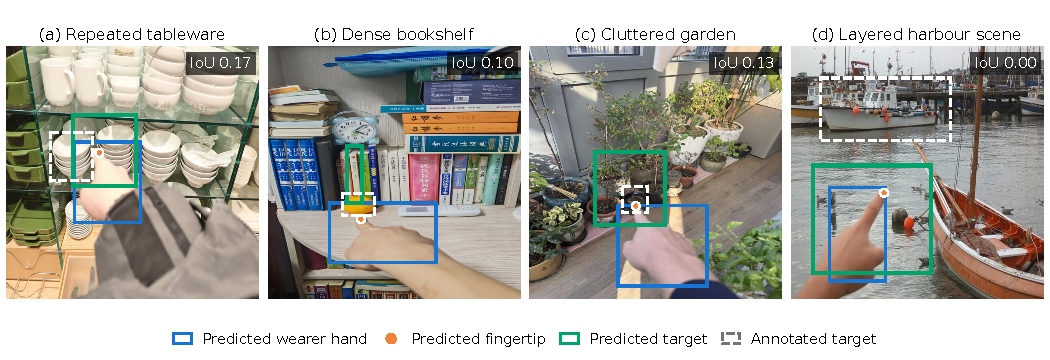
\includegraphics[width=\linewidth]{figures/failures_complex}
  \caption{Selected complex failures: repeated tableware (a) and a dense bookshelf (b) create look-alike neighbours; foliage complicates the target's extent (c); several depth layers separate the fingertip from the labelled boat (d). Colours as in Figure~\ref{fig:teaser}; boxes, points and IoUs are the saved test predictions of the 160\,px model.}
  \Description{Four egocentric photos where the predicted target box misses the labelled one: a box on the wrong stack of tableware in a glass cabinet (IoU 0.17), a box on a neighbouring book in a dense bookshelf (IoU 0.10), a box covering plants around a small object in a garden (IoU 0.13), and a foreground box instead of a distant boat in a harbour (IoU 0.00). The wearer's hand and fingertip are found in all four.}
  \label{fig:failures}
\end{figure}

\section{Discussion}\label{sec:discussion}

\paragraph{Design implications.} For pointing interfaces on glasses, our results suggest five practical rules.
\begin{enumerate}
\item \emph{Choose the model by what the interface needs.} For a tight target box, a compact detector trained on pointing data is more accurate at the same compute. For naming the target, a structured model does as well, and it also provides the hand, the fingertip and the direction for feedback or gating in the same pass (Section~\ref{sec:choice}).
\item \emph{Train with distractor hands, whatever the model.} Pasting unlabelled hands into the training images makes SpatialNet and a generic detector equally stable when hands are pasted into the view, at no cost on clean images (Section~\ref{sec:design}).
\item \emph{Spend extra compute on resolution first.} A larger input gained more than a larger backbone (Section~\ref{sec:design}).
\item \emph{Confirm before acting.} Errors concentrate where similar objects lie side by side or the target is far from the fingertip, and single frames produce false alarms. Naming or highlighting the target before acting, and requiring several consecutive detections, protect the wearer from both (Section~\ref{sec:failures}).
\item \emph{Keep frames on the device.} A later recogniser needs only the target crop (Section~\ref{sec:choice}), which limits computation, bandwidth and the bystander imagery that leaves the glasses. Whether local inference also saves energy needs repeated measurements; the single observations of Section~\ref{sec:ondevice} only point in that direction.
\end{enumerate}

\paragraph{Limitations.} \emph{Data.} All accuracy figures except Section~\ref{sec:realframes} come from one dataset whose images are mostly landscape, partly composed or edited, at least 41\% derived from COCO, and in 4.7\% of test cases duplicated in the training or validation split (Appendix~\ref{app:data}); its demographic coverage is unknown. Frames are squashed to a square, whereas the glasses' camera is portrait. EgoPoint has no non-pointing hands and no pointing without a target, so the pointing and target gates are untested, and in deployment a non-pointing hand may be read as pointing. The model has no temporal context. \emph{Other hands.} Our distractors are synthetic and encode the prior that the wearer's arm enters from the bottom of the view; real bystander hands are untested. \emph{Evidence.} The ablations, the resolution runs and three of the four controlled detector runs are single training runs, and the per-component reading of the ablations is exploratory. We copied the large-model results rather than re-running them. The recognition test is category-level and uses zero-shot recognisers. The device results are single observations on a pre-production unit, and the detectors were not measured on the glasses. \emph{Interaction.} We measured the model, not the interaction: how wearers respond to its errors, and which confirmation designs suit them, needs a study with participants wearing the glasses.

\section{Ethics and Privacy}\label{sec:ethics}

\paragraph{Bystanders.} A head-worn camera sees people who did not consent to being recorded, and bystanders' concerns about camera glasses are well documented~\cite{denning2014situ,hoyle2014privacy}. SpatialNet runs on the glasses, so localisation needs no frame to leave the device, and a later step can be limited to the target crop and to moments when the wearer points. SpatialNet is trained to ignore other people's hands; it does not detect, identify or track people. On-device processing does not remove the need for visible recording indicators; the test unit has user- and bystander-facing LEDs.

\paragraph{Data.} EgoPoint is used under the access terms of its authors' release, for research only. We do not redistribute its images or our converted labels; our conversion script regenerates the labels from the original release. The images shown in this paper come from its test and training splits. \tbd{Real-frame check (Section~\ref{sec:realframes}): state who recorded the frames and how they consented, the ethics approval or exemption, how long the frames are kept, and how bystanders were kept out of view or blurred.}

\paragraph{Availability.} We will release the code, the dataset conversion script, the trained weights and the per-image evaluation outputs, from which every table can be recomputed, upon publication.

\section{Conclusion}\label{sec:conclusion}
SpatialNet localises the object a smart-glasses wearer points at from a single RGB frame, with one forward pass of a 0.72M-parameter CNN and no prompt, language model or external hand model, and it runs on a pre-production pair of glasses in 60--80\,ms per frame. It is far less accurate than large GPU models, and compact detectors of the same compute draw tighter boxes. But it picks the labelled object more often than those detectors, a recogniser names the object from its crops as often as from theirs, and it returns the hand, the fingertip and the direction from the same pass. At this scale, input resolution is the largest lever, instance anchoring sharpens the hand box and the direction, training with distractor hands carries over to other models, and an explicit ray prior is not needed. At least 41\% of the EgoPoint test images are COCO photographs, which benchmarks on this dataset should take into account. The main open problems are pointing scenes that EgoPoint does not contain, real bystander hands, and evidence that on-device pointing helps people in daily use.


\bibliographystyle{ACM-Reference-Format}
\bibliography{references,references-revision}

\appendix
\section{Method Details}\label{app:method}
\paragraph{Training schedule.} We train with AdamW~\cite{loshchilov2019decoupled} (weight decay $10^{-4}$, batch size 32) and a one-cycle schedule~\cite{smith2019super} (peak learning rate $3\times10^{-3}$ for the heads and $3\times10^{-4}$ for the backbone, 10\% warm-up, then cosine decay) for up to 180 epochs, stopping early after 25 epochs without a lower validation loss, with gradient clipping at 1.0, mixed precision and seed 42. Training took 1\,h\,40\,min on one NVIDIA Tesla T4 (47\,s per epoch). Early stopping ended it after 125 epochs, before the one-cycle schedule had completed; the reported checkpoint, the one with the lowest validation loss, is from epoch 100. Every run in this paper uses the same stopping rule, but runs stop at different epochs, which we take into account when comparing them. The model is exported to ONNX (opset 17, which bilinear grid sampling requires) and to FP16.

\subsection{Augmentation}\label{app:aug}
Besides the distractor pasting of Section~\ref{sec:ownership}, we use horizontal flips (but no vertical flips, because a wearer's hand entering from the top would contradict the ownership prior), shift, scale and rotation, perspective warps, brightness and contrast changes, Gaussian blur, and mixup~\cite{zhang2018mixup} between images of the same scene. With probability 0.15, we also paste an unlabelled patch that contains no hand, so that a pasted rectangle is not itself a cue. In the hand-heatmap loss, the negative term near a pasted hand is multiplied by $1+4\,G_k$, where $G_k$ is a Gaussian ($\sigma{=}1.5$ cells) at that hand's centre. Table~\ref{tab:aug} lists all settings.

\begin{table}[h]
  \caption{Training-time augmentation, applied on the fly; each training image is seen once per epoch as a new random variant. Validation and test images are only resized and normalised.}
  \label{tab:aug}
  \footnotesize
  \begin{tabular}{lp{0.62\linewidth}}
    \toprule
    Step & Setting \\
    \midrule
    Distractor hands & 1--2 hands with probability 0.5 (hand images) or 0.3 (no-hand images); scale 0.45--1.0; rotation by 90/180/270$^\circ$ and optional mirror with probability 0.7; centre in the top 65\% of the frame; overlap with the wearer's hand and the target below 15\%; feathered alpha (12\% of the crop size); colour jitter; 30\% self-paste; pool of 512 donor crops, half from pointing hands \\
    Decoy patch & unlabelled non-hand patch from a no-hand image, with probability 0.15 \\
    Horizontal flip & 0.5 \\
    Shift / scale / rotate & ${\pm}5\%$ / ${\pm}10\%$ / ${\pm}15^\circ$, probability 0.4 \\
    Perspective & scale 0.02--0.05, probability 0.2 \\
    Brightness / contrast & ${\pm}20\%$, probability 0.5 \\
    Gaussian blur & kernel 3--5, probability 0.2 \\
    Mixup & within the same scene, $\lambda\sim\mathrm{Beta}(0.2,0.2)$ folded to ${\geq}0.5$, label of the dominant image, every batch \\
    Anchor forcing & ground-truth anchors with probability 0.5 decaying to 0 over 20 epochs \\
    \bottomrule
  \end{tabular}
\end{table}

\section{Data}\label{app:data}

\paragraph{EgoPoint.} The EgoPoint-Ground paper~\cite{egopoint} reports 15,338 images: 39\% (6,035) real captures with smart glasses, 39\% (5,976) synthetically composed and 22\% (3,327) generated by editing; its appendix calls the last two groups ``synthetic generation'' and ``image editing''. The edited images were made from third-person photographs of COCO~\cite{lin2014coco}, selected through the RefCOCO referring-expression dataset~\cite{yu2016modeling}, into which a multimodal model added a pointing hand. The release we use has 15,455 images split 10,837 / 1,546 / 3,072. VistaRef~\cite{li2026vistaref} and PointVG-R~\cite{li2026pointvgr} report the same counts, so our test images are theirs, minus the exclusions below. Each positive record shows one wearer's hand pointing at one target; negatives show no hand.

\paragraph{Conversion.} Negatives become scene 000 (no hand), and their object boxes are ignored; positives with a hand box, an annotated fingertip and a target box become scene 111 (pointing at a target). In three test records, the hand label was attached to an object and the hand was labelled as an object; we detected these by the fingertip position and swapped the labels back. We dropped 232 positives: 229 without an annotated fingertip (164 train, 22 validation, 43 test), all flagged as unclear in the source annotations, and 3 without a hand box. Spot checks showed open palms, held objects, or a hand box on the hand that was not pointing. If all 43 dropped test positives were counted as failures, the target P@0.5 would fall by less than one point, to about 58\%. Images are stored at $224\times224$; the model squashes every frame to its square $160\times160$ input, regardless of the original aspect ratio. Table~\ref{tab:data} summarises the result.

\paragraph{Fingertip--target gap.} We describe each target by its gap to the fingertip in the image: \emph{overlap} when the fingertip lies inside the target box, \emph{near} when the shortest fingertip--box distance is at most 0.08 of the image side, and \emph{large gap} otherwise. These are image-plane relations: an overlap does not imply that the finger touches the object, and a large gap does not imply that the object is far from the wearer. About 70\% of targets overlap the fingertip and only 7\% have a large gap, so pooled results are dominated by overlap targets; Appendix~\ref{app:heads} reports the main metrics by gap.

\begin{table}[h]
  \caption{EgoPoint after conversion, by split, scene and fingertip--target gap.}
  \label{tab:data}
  \footnotesize
  \begin{tabular}{lrrrrrr}
    \toprule
    & & & & \multicolumn{3}{c}{Pointing at target, by gap} \\
    \cmidrule(l){5-7}
    Split & Images & No hand (000) & Pointing at target (111) & Overlap & Near & Large gap \\
    \midrule
    Train & 10,669 & 1,535 & 9,134 & 6,511 & 1,995 & 628 \\
    Validation & 1,524 & 211 & 1,313 & 922 & 297 & 94 \\
    Test & 3,029 & 425 & 2,604 & 1,796 & 599 & 209 \\
    \midrule
    Total & 15,222 & 2,171 & 13,051 & 9,229 & 2,891 & 931 \\
    \bottomrule
  \end{tabular}
\end{table}

\paragraph{COCO overlap.} The release names the source photograph of each edited image. In our test split, 842 of the 2,604 images with a target (32\%) are edited COCO train2014 photographs, and at least 400 of the 425 no-hand images are unedited COCO train2014 photographs, so at least 1,242 test images (41\%) come from COCO. COCO-pretrained detector weights are trained on COCO train2017, which contains every train2014 photograph, together with box annotations of the objects they contain. In addition, 230 test images share their COCO source photograph with a training or validation image; this overlap within EgoPoint affects all trained models alike.

\paragraph{Near-duplicates.} 141 test images (4.7\%) are byte-identical to a training or validation image, and 362 have an exact or near copy there. We therefore repeat the headline comparisons on the test split without the 141 duplicates. Unless stated otherwise, every conclusion holds on that duplicate-free set; the main model's P@0.5 moves from 58.9\% to 57.2\%, inside its confidence interval.

\paragraph{Model selection.} Training, early stopping and checkpoint selection use only the training and validation splits; the test split is evaluated once, after training. The ablation, resolution and seed runs follow the same rule and do not change the reported model.

\section{Additional Results}\label{app:extra}

\subsection{Comparison with Published Models and the Benchmark Detectors}\label{app:comparison}

Table~\ref{tab:main-full} extends Table~\ref{tab:main}. VistaRef and PointVG-R report results on the same 3,072-image test split, from which ours omits 43 unclear images and the 425 images without a target; PointVG-R also reports zero-shot and fine-tuned multimodal LLMs on that split. EgoPoint-Ground's pointing-only (POG) results come from a different setting: zero-shot models receive the ground-truth hand box, and the evaluated subset is not stated. Three simple references test whether knowing where the fingertip is would be enough: the mean training target box at a fixed position, and a box of mean training size centred on SpatialNet's predicted fingertip or on the ground-truth fingertip. A mean-size box at the true fingertip reaches a P@0.5 of only 11.4\% (12.0\% when shifted by the mean training offset), because target sizes vary widely (2.6\% to 44\% of the image area, 10th to 90th percentile).

Against zero-shot multimodal LLMs the picture is mixed. SpatialNet's P@0.5 and mIoU are above those reported for zero-shot Qwen2.5-VL-7B and Qwen3-VL-8B, and its P@0.3 is far higher, but the zero-shot models draw tighter boxes (P@0.7 of 39.0--42.9\% against 31.8\%), and models given the true hand box reach 61.2--63.9\% P@0.5. Because the published rows count IoU${>}\tau$, include no-target images scored in an unstated way and, in one case, use an unstated subset, and because models trained on large image collections may also have seen COCO, we read this as the same accuracy range at a fraction of the size, not as parity or superiority.

\begin{table}[h]
  \caption{Localisation of the pointed-at target on the EgoPoint test split. Our rows use the 2,604 test images with a target. mIoU and P@$\tau$ in \%, the published values multiplied by 100. We count IoU${\geq}\tau$, as does VistaRef; EgoPoint-Ground and PointVG-R count IoU${>}\tau$. \emph{Large gap}: P@0.5 on the 209 large-gap targets.
  $^\ast$\,VistaRef~\cite{li2026vistaref}, Table~1, setting ``Train-Real Data Test'', BEiT-3-L backbone (226M parameters with BEiT-3-Base); test set of 3,072 images, which includes no-hand images.
  $^\ddagger$\,PointVG-R~\cite{li2026pointvgr}, Table~1, EgoPoint-CoT test set, built on the same release and test split.
  $^\dagger$\,EgoPoint-Ground~\cite{egopoint}, Table~4, pointing-only (POG) task: inference only, given the ground-truth hand box; the evaluated subset is not stated.
  How the published works score images without a target is not stated; if they counted the 425 no-target images as failures, zero-shot Qwen2.5-VL-7B would reach about 57.8\% P@0.5 and 52.8\% mIoU on the images with a target.}
  \label{tab:main-full}
  \footnotesize
  \setlength{\tabcolsep}{3.4pt}
  \begin{tabular}{lrrrrrr}
    \toprule
    Method & Params & P@0.3 & P@0.5 & P@0.7 & mIoU & Large gap \\
    \midrule
    \multicolumn{7}{l}{\emph{Published, trained on EgoPoint (not re-run)}} \\
    \quad VistaRef$^\ast$, image + fixed prompt & $>$226M & 97.0 & 93.9 & 82.6 & 82.0 & -- \\
    \quad PointVG-R$^\ddagger$, image + instruction, SFT + RL & 7B & 88.1 & 83.6 & 74.5 & 75.7 & -- \\
    \quad Qwen2.5-VL-7B$^\ddagger$, image + instruction, SFT & 7B & 68.7 & 63.6 & 56.7 & 59.8 & -- \\
    \multicolumn{7}{l}{\emph{Published, zero-shot (not re-run)}} \\
    \quad Qwen2.5-VL-7B$^\ddagger$, image + instruction & 7B & 54.2 & 49.8 & 42.9 & 45.5 & -- \\
    \quad Qwen3-VL-8B$^\ddagger$, image + instruction & 8B & 48.1 & 44.5 & 39.0 & 43.0 & -- \\
    \quad SV-CoT$^\dagger$, image + hand box & $>$1B & 69.4 & 63.9 & 55.6 & -- & -- \\
    \quad Qwen3-VL-4B$^\dagger$, image + hand box & 4B & 67.1 & 61.2 & 53.2 & -- & -- \\
    \multicolumn{7}{l}{\emph{Simple references}} \\
    \quad Mean training box, fixed position & 0 & 41.3 & 9.6 & 0.9 & 27.4 & 4.3 \\
    \quad Mean-size box at predicted fingertip & 0.72M & 43.5 & 11.2 & 0.9 & 28.8 & 0.0 \\
    \quad Mean-size box at true fingertip (oracle) & -- & 43.6 & 11.4 & 1.0 & 29.0 & 0.0 \\
    \midrule
    \textbf{SpatialNet} (image only, seed 42) & 0.72M & 78.6 & 58.9 & 31.8 & 53.3 & 25.4 \\
    \quad mean $\pm$ std, 3 seeds & & 78.1{\scriptsize$\pm$0.6} & 59.0{\scriptsize$\pm$0.1} & 31.5{\scriptsize$\pm$0.4} & 52.9{\scriptsize$\pm$0.5} & 26.3{\scriptsize$\pm$1.3} \\
    \bottomrule
  \end{tabular}
\end{table}

\paragraph{Benchmark of compact detectors.} Table~\ref{tab:detectors} compares SpatialNet with YOLO26n and NanoDet-Plus-m from several starting points, trained on the same split and scored with the same code, plus higher-resolution runs of both. \tbd{State the benchmark detectors' training recipe: classes, epochs, augmentation, how one hand box and one target box are selected per image, and the validation rule used to tune the hand-gate thresholds of the end-to-end score.} GFLOPs are counted with the same \texttt{torch} FLOP counter; model sizes are the serialised SpatialNet state dicts and the exported ONNX files of the detectors, of which we count only the inference parameters. With the same ImageNet pretraining as our backbone, YOLO26n is 4.3 points ahead in P@0.5, mostly in tight boxes (P@0.7 +10.6) and large-gap targets (+11.4), and its hand mIoU is 7.4 points higher; trained from scratch, it is 1.0 point ahead.

\paragraph{End-to-end score.} The target metrics ignore the gates. The end-to-end score covers all 3,029 test images: a target image counts as correct if the hand gate fires, the model predicts ``pointing at target'' and the target box has IoU${\geq}0.5$; a no-hand image counts as correct if the model says ``no hand''. Each model's hand-gate threshold is tuned on the validation split by the same rule. Counting the gate costs each model 0.3--1.3 points of P@0.5, and every model rejects 95.3--98.4\% of no-hand frames, so the order does not change: SpatialNet reaches 63.6\%, on a par with YOLO26n from scratch (63.8\%) and below YOLO26n with an ImageNet start (67.4\%) and the COCO-pretrained detectors (68.9--71.1\%). On the test split without duplicates the order is the same.

\begin{table}[h]
  \caption{SpatialNet and the benchmark detectors, trained on EgoPoint and scored by the same code (\%, on the 2,604 test images with a target, except \emph{End-to-end}, which covers all 3,029 test images). \emph{Pasted}: change in target P@0.5 when one or two hands are pasted into each test image; none of these detectors was trained with pasted hands. $^\dagger$\,Pretrained on COCO train2017.}
  \label{tab:detectors}
  \footnotesize
  \setlength{\tabcolsep}{3pt}
  \begin{tabular}{lrrrrrrrrrr}
    \toprule
    Model & Params & GFLOPs & P@0.5 & P@0.7 & mIoU & Large & Hand & Centre & Pasted & End-to- \\
    & & & & & & gap & mIoU & in & & end \\
    \midrule
    \multicolumn{11}{l}{\emph{Matched compute}} \\
    SpatialNet, 160\,px, ImageNet & 0.72M & 0.231 & 58.9 & 31.8 & 53.3 & 25.4 & 73.7 & 84.8 & $+$1.2 & 63.6 \\
    YOLO26n, 128\,px, scratch & 2.50M & 0.225 & 59.9 & 39.1 & 54.7 & 31.6 & 80.6 & 81.6 & $-$4.6 & 63.8 \\
    YOLO26n, 128\,px, ImageNet & 2.50M & 0.225 & 63.2 & 42.4 & 56.8 & 36.8 & 81.1 & 82.3 & $-$3.6 & 67.4 \\
    YOLO26n, 128\,px, COCO$^\dagger$ & 2.50M & 0.225 & 65.0 & 47.0 & 58.6 & 39.7 & 81.6 & 82.2 & $-$4.0 & 68.9 \\
    NanoDet-Plus-m, 160\,px, COCO$^\dagger$ & 1.17M & 0.218 & 67.6 & 49.5 & 59.8 & 40.7 & 81.5 & 82.9 & $-$4.5 & 71.1 \\
    \midrule
    \multicolumn{11}{l}{\emph{Higher compute}} \\
    SpatialNet, 224\,px, ImageNet & 0.72M & 0.453 & 62.4 & 37.1 & 54.8 & 35.9 & 74.9 & 83.7 & $+$1.5 & 66.8 \\
    SpatialNet, 320\,px, ImageNet & 0.72M & 0.923 & 65.1 & 40.3 & 56.5 & 34.9 & -- & -- & -- & 69.3 \\
    YOLO26n, 160\,px, COCO$^\dagger$ & 2.50M & 0.352 & 66.9 & 48.8 & 60.3 & 42.1 & 82.1 & 83.5 & $-$3.0 & 70.8 \\
    YOLO26n, 192\,px, COCO$^\dagger$ & 2.50M & 0.507 & 69.9 & 53.3 & 62.8 & 43.5 & 82.9 & 84.7 & $-$2.6 & 73.6 \\
    \bottomrule
  \end{tabular}
\end{table}

\subsection{Controlled Detector Runs}\label{app:controlled}

We trained YOLO26n ourselves under one fully specified recipe (Ultralytics 8.4.177): the converted EgoPoint images at $128\times128$; two classes, the wearer's hand and the target, with no labels on no-hand images; 150 epochs with early stopping after 50 epochs without improvement, batch 64; and Ultralytics' default augmentation without mosaic, mixup or copy-paste. The backbone starts from ImageNet (the YOLO26n classification weights, which initialise its first ten layers, with the neck and head from scratch) or from COCO. One ImageNet-start run is also trained with our distractor pasting, applied on the fly with the same code and probabilities as for SpatialNet; the pasted hands stay unlabelled background, since a detector has no ownership-weighted heatmap loss. For each image we score the top-scoring hand box and target box, and for every model, SpatialNet included, the hand-gate threshold is the value that maximises no-hand versus hand accuracy on the validation split (Table~\ref{tab:controlled}).

The ImageNet-start run reproduces the benchmark (62.9\% against 63.2\% P@0.5), and its second seed differs from it by 0.6 points ([$-$1.0, +2.2]). Against the first seed, SpatialNet is 4.0 points lower in P@0.5 ([$-$6.0, $-$2.2]) and 11.6 lower in P@0.7 ([$-$13.4, $-$9.6]); against the second, 4.6 and 11.5 points lower. Its predicted target centre lies inside the labelled box more often than for every run: the paired differences are 2.8 [1.4, 4.1] and 3.2 [1.8, 4.6] points against the two ImageNet-start seeds, 3.0 [1.7, 4.5] against the run with pasting and 2.6 [1.3, 4.0] against the COCO start.

\paragraph{Robustness to other hands comes from the training recipe.} Trained without pasting, the detectors lose 2.4--4.1 points of P@0.5 when hands are pasted into the test images and keep only 87.8--88.7\% of no-hand frames, whereas SpatialNet gains 1.2 points and keeps 96.7\%. Trained with our pasting, the same YOLO26n is as stable as SpatialNet: it changes by $+$0.7 points (difference from SpatialNet $-$0.6 [$-$2.2, $+$0.8]) and keeps 95.8\% of no-hand frames ($-$0.9 [$-$3.8, $+$1.4]). Pasting improves the detector's change under interference by 3.8 points [2.4, 5.2] and the no-hand frames kept by 8.0 [5.2, 10.8], at no cost on clean images (P@0.5 $+$0.3 [$-$1.2, $+$1.8]).

\paragraph{COCO pretraining does not exploit the overlap.}\label{app:coco} If COCO pretraining helped mainly by having seen the test sources, its gain would concentrate on the 842 COCO-derived test images. It does the opposite: against the ImageNet start, the COCO start gains 2.4 points [0.6, 4.3] on the other test images and $-$0.7 [$-$3.7, $+$2.5] on the COCO-derived ones (difference $-$3.2 [$-$6.7, $+$0.3]). NanoDet-Plus-m was not retrained, so this test covers YOLO26n only. All models, SpatialNet included, find the COCO-derived images harder (51.8--56.1\% against 62.3--68.7\% P@0.5).

\begin{table}[h]
  \caption{SpatialNet and four controlled YOLO26n runs (128\,px), scored by the same code on the same test images (\%). \emph{Pasted}: change in target P@0.5 with one or two pasted hands per image. \emph{No hand kept}: no-hand images still classed as no hand when hands are pasted into them, at validation-tuned thresholds. \emph{COCO} and \emph{Other}: P@0.5 on the 842 test images made from COCO train2014 photographs and on the remaining 1,762.}
  \label{tab:controlled}
  \footnotesize
  \setlength{\tabcolsep}{2.6pt}
  \begin{tabular}{lrrrrrrrrr}
    \toprule
    & & & Large & Hand & Centre & & No hand & \multicolumn{2}{c}{P@0.5, source} \\
    \cmidrule(l){9-10}
    Model & P@0.5 & P@0.7 & gap & mIoU & in & Pasted & kept & COCO & Other \\
    \midrule
    \textbf{SpatialNet} (ImageNet) & 58.9 & 31.8 & 25.4 & 73.7 & \textbf{84.8} & $+$1.2 & 96.7 & 51.8 & 62.3 \\
    YOLO26n, ImageNet & 62.9 & 43.4 & 36.8 & 81.0 & 82.1 & $-$3.1 & 87.8 & 56.1 & 66.2 \\
    YOLO26n, ImageNet, seed 1 & 63.6 & 43.3 & 38.3 & 81.0 & 81.6 & $-$4.1 & 88.7 & 54.9 & 67.7 \\
    YOLO26n, ImageNet + pasting & 63.2 & 42.7 & 36.8 & 80.9 & 81.8 & $+$0.7 & 95.8 & 55.5 & 66.9 \\
    YOLO26n, COCO & 64.4 & 45.5 & 36.4 & 81.4 & 82.2 & $-$2.4 & 87.8 & 55.3 & 68.7 \\
    \bottomrule
  \end{tabular}
\end{table}

\paragraph{Ownership under pasted hands.} With one or two hands pasted into each test image (Table~\ref{tab:own}), SpatialNet's hand lies nearer the wearer's hand than any pasted hand in 99.7\% of hand images, and its target P@0.5 does not drop. This ownership metric is easy under the synthetic distribution: pasted hands sit in the upper part of the frame and the wearer's hand in the lower part, so ownership accuracy on training batches was already 93\% in the first epoch. The no-hand frames kept and the target accuracy under interference are more informative, and both need the pasting recipe (ablation A1).

\begin{table}[h]
  \caption{Ownership on test images with one or two pasted hands (\%). \emph{On other hand}: predicted hand centre inside a pasted hand. \emph{No hand kept}: no-hand images still classed as no hand, at the hand-gate threshold of 0.5.}
  \label{tab:own}
  \footnotesize
  \begin{tabular}{lrrrr}
    \toprule
    & Ownership accuracy & On other hand & No hand kept & Target P@0.5 \\
    \midrule
    Full model, clean test images & -- & -- & 93.4 & 58.9 \\
    Full model, pasted hands & 99.7 [99.4, 99.9] & 0.2 & 91.8 & 60.1 \\
    A1 (no pasting), pasted hands & 98.7 [98.2, 99.1] & 1.2 & 86.4 & 56.1 \\
    \bottomrule
  \end{tabular}
\end{table}

\subsection{Per-Head Accuracy and Hand Presence}\label{app:heads}

\begin{table}[h]
  \caption{Accuracy of each head by fingertip--target gap (test split, pointing-at-target images). Fingertip error in pixels at the $160\times160$ input; direction error in degrees. mIoU and P@0.5 in \%; brackets: 95\% bootstrap confidence intervals of the mIoU.}
  \label{tab:heads}
  \footnotesize
  \setlength{\tabcolsep}{4pt}
  \begin{tabular}{lrrrrrrrr}
    \toprule
    & \multicolumn{2}{c}{Hand} & \multicolumn{2}{c}{Fingertip (px)} & \multicolumn{2}{c}{Direction ($^\circ$)} & \multicolumn{2}{c}{Target} \\
    \cmidrule(lr){2-3}\cmidrule(lr){4-5}\cmidrule(lr){6-7}\cmidrule(l){8-9}
    Gap (images) & mIoU & P@0.5 & mean & ${<}5$\,px & mean & ${<}15^\circ$ & mIoU [CI] & P@0.5 \\
    \midrule
    Overlap (1,796) & 73.7 & 92.3 & 3.79 & 84.4 & 36.0 & 39.7 & 57.9 [56.8, 59.0] & 66.0 \\
    Near (599) & 73.7 & 93.5 & 4.09 & 78.8 & 22.0 & 54.9 & 47.8 [45.8, 49.8] & 49.2 \\
    Large gap (209) & 72.7 & 92.8 & 4.16 & 80.9 & 29.0 & 36.8 & 29.8 [26.0, 33.6] & 25.4 \\
    \midrule
    All (2,604) & 73.7 & 92.6 & 3.89 & 82.8 & 32.2 & 43.0 & 53.3 [52.3, 54.3] & 58.9 \\
    \bottomrule
  \end{tabular}
\end{table}

\paragraph{Where the errors come from.} The hand box and fingertip are equally good at every gap (hand P@0.5 of 92--94\%; about 4\,px fingertip error, 2.5\% of the image side), so they are not the bottleneck. The target falls off with the gap: P@0.5 drops from 66.0\% for overlap targets to 49.2\% for near and 25.4\% for large-gap ones (Table~\ref{tab:heads}). The direction is coarse: its median error is 18.6$^\circ$, and only 36.8\% of large-gap targets have an error below 15$^\circ$. At their median fingertip--target distance of 0.32 image widths, 15$^\circ$ already moves the ray by about 0.08 image widths, the size of a small object. The error is largest for overlap targets (36$^\circ$), where the direction to the target centre is ill-defined and matters least. Position and extent errors contribute about equally: giving the model the true size with its own centre would raise P@0.5 to 70.4\%, and giving it the true centre with its own size would raise it to 72.3\%. Size is regressed towards the mean: small targets (under 3\% of the image) are predicted about 1.9 times too large and reach a P@0.5 of only 36.9\% (27.8--36.9\% across seeds).

\paragraph{Hand presence.} The hand gate separates no-hand from pointing frames with 98.6\% accuracy (95\% CI 98.1--98.9) and AUROC 0.998. At threshold 0.5, it misses 15 of 2,604 hands (0.6\%) and raises false alarms on 28 of 425 no-hand frames (6.6\%). Choosing the threshold on validation so that no hand is missed (0.22) would raise false alarms to 117 (27.5\%), so we keep 0.5. Per-frame false alarms of this size mean that an always-on interface needs temporal smoothing, for example requiring several consecutive detections, which we do not evaluate.

\subsection{Recognition Test}\label{app:recog}

\paragraph{Protocol.} For each of the 2,603 test targets with a category name, we crop the predicted target box of each model from the 320\,px copy of the image, restore the photograph's original aspect ratio, pad the crop to a square and classify it zero-shot among the 348 target category names of EgoPoint, averaging four prompt templates (``a photo of a \{\}.'' and three variants). Crops of the labelled box and of the whole frame are references. The test is category-level: a box on a neighbouring object of the same category counts as recognised, and near-synonyms such as ``bike'' and ``bicycle'' count as errors, for every model alike. Both recognisers ran on CPU; larger recognisers (CLIP ViT-L/14, SigLIP so400m) were planned on a GPU, but those runs did not complete.

\paragraph{Further results.} Top-5 accuracy gives the same result as top-1 (differences from $-$1.3 to 0.0 points; one interval of eight excludes zero, by 0.04 points), and so do SpatialNet's seeds 1 and 2 (48.3--49.1\% and 52.5--52.6\% top-1). When SpatialNet's box misses IoU 0.5 but its centre lies on the labelled object, the crop is still named correctly in 47--51\% of cases, against 54--58\% for boxes with IoU${\geq}0.5$ and 30\% when the centre misses. Large-gap targets are the exception (Table~\ref{tab:recog-full}): there, the detectors' crops are named correctly 4.3--8.1 points more often than those of the deployed model (the interval excludes zero in five of the eight comparisons; seeds 1 and 2 of SpatialNet lie in between, at 37.3--43.1\%), and its crops are named about as often as the whole frame, or less often. Restricting the test to targets other than people, 20\% of the test set, changes no difference by more than one point.

\begin{table}[h]
  \caption{Recognition test with the large-gap subset (top-1 accuracy, \%; 2,603 test targets, 209 of them with a large gap).}
  \label{tab:recog-full}
  \footnotesize
  \begin{tabular}{lrrrr}
    \toprule
    & \multicolumn{2}{c}{CLIP ViT-B/16} & \multicolumn{2}{c}{SigLIP base} \\
    \cmidrule(lr){2-3}\cmidrule(l){4-5}
    Crop & All & Large gap & All & Large gap \\
    \midrule
    Labelled box (upper reference) & 53.9 & 51.2 & 59.4 & 54.1 \\
    Whole frame (lower reference) & 40.3 & 33.5 & 46.2 & 43.1 \\
    \midrule
    \textbf{SpatialNet} (seed 42) & 48.6 & 34.9 & 52.3 & 36.8 \\
    YOLO26n, ImageNet & 48.8 & 43.1 & 53.3 & 41.6 \\
    YOLO26n, ImageNet, seed 1 & 49.1 & 41.1 & 53.4 & 41.1 \\
    YOLO26n, ImageNet + pasting & 49.9 & 43.1 & 52.0 & 43.5 \\
    YOLO26n, COCO & 49.1 & 42.1 & 53.2 & 42.1 \\
    \bottomrule
  \end{tabular}
\end{table}

\subsection{Input Resolution}\label{app:resolution}

A convolutional network shares its filters across positions, so a larger input costs compute but no parameters. We retrained the unchanged model (722,104 parameters, same seed and settings) at 224\,px, using the stored $224\times224$ images at full resolution instead of downsampling them, and at 320\,px, re-converting the dataset from the original images so that the larger input carries real detail rather than upsampled pixels (Table~\ref{tab:detectors}). From 160 to 320\,px, P@0.5 rises by 6.2 points (95\% paired-bootstrap CI [+4.4, +8.0]) to 65.1\%, P@0.7 by 8.5 points [+6.8, +10.3] and mIoU by 3.2, and the fingertip error falls from 2.43\% to 1.32\% of the image width; 224\,px lies in between. Large-gap targets gain first and then stop (25.4\% at 160\,px, 35.9\% at 224\,px, 34.9\% at 320\,px), while the mean direction error is flat at every resolution (31.4--32.2$^\circ$). With one run per resolution, this suggests, but does not show, that the direction estimate rather than the input limits large-gap targets beyond 224\,px. Small targets gain only at 320\,px (36.9\% $\to$ 46.6\% P@0.5), where the images were re-converted from the originals. Both higher-resolution runs stopped early at 84 epochs (best epoch 59, against 100 at 160\,px), so their gains may be underestimated. Compute grows from 0.23 to 0.45 and 0.92 GFLOPs (CPU latency on the evaluation machine 25.7, 37.2 and 50.8\,ms), while the weights stay at 1.6\,MB.

\subsection{Ablations}\label{app:ablation}

We retrain the 160\,px model without one component at a time, with the seed and settings of the main run: \textbf{A1} no distractor pasting and no ownership weighting; \textbf{A2} no geometric consistency terms; \textbf{A3} no ray conditioning of the target head (no $G^t$; 13,105 fewer parameters); \textbf{A4} no instance-anchored chain, so that the direction head and gates read the globally pooled vector and the fingertip has no hand-anchored terms, which gives a plain model of the same size (709K parameters). Each ablation was trained once, and we test each difference in two ways: a paired bootstrap over test images gives a 95\% interval for test-sample variation, and retraining the full model with two more seeds gives the training variation. A difference counts as an effect only if its interval excludes zero \emph{and} it exceeds the largest change that retraining alone produced (Table~\ref{tab:ablation-full}, second row). With one seed per variant and several metrics per component, we treat these comparisons as exploratory. Figure~\ref{fig:ablation} shows, for each component, the metrics it was designed to improve.

\begin{table}[h]
  \caption{Ablations at 160\,px, all metrics (one seed each). First row: the full model; other rows: difference from it (points, or degrees for the direction error, where positive means worse). Bold: the 95\% paired interval excludes 0 and the difference exceeds the retraining row. $^\S$\,Not significant on the duplicate-free test split. \emph{Small}: targets under 3\% of the image (309 images).}
  \label{tab:ablation-full}
  \footnotesize
  \setlength{\tabcolsep}{3pt}
  \begin{tabular}{lrrrrrrrrr}
    \toprule
    & \multicolumn{7}{c}{Clean test images} & \multicolumn{2}{c}{With other hands} \\
    \cmidrule(lr){2-8}\cmidrule(l){9-10}
    Variant & mIoU & P@0.5 & P@0.7 & Large gap & Small & Hand & Dir.\,($^\circ$) & P@0.5 & No hand \\
    \midrule
    Full model & 53.3 & 58.9 & 31.8 & 25.4 & 36.9 & 73.7 & 32.2 & 60.1 & 91.8 \\
    \quad Retraining (seeds 1, 2) & $\pm$0.9 & $\pm$0.1 & $\pm$0.8 & $\pm$2.4 & $\pm$9.1 & $\pm$0.3 & $\pm$1.2 & $\pm$0.4 & $\pm$3.3 \\
    \midrule
    A1 no hand pasting & \textbf{$-$1.2} & $-$0.1 & $-$1.3 & $+$1.9 & $-$3.9 & \textbf{$-$0.6} & \textbf{$+$1.8} & \textbf{$-$4.1} & \textbf{$-$5.4} \\
    A2 no ray / axis losses & $-$0.5 & $+$1.1 & $+$0.6 & $+$3.3 & $-$0.6 & $-$0.4 & \textbf{$+$1.5} & 0.0 & $-$1.2 \\
    A3 no ray conditioning & $+$0.2 & $+$0.7 & \textbf{$+$1.9}$^\S$ & $+$5.3 & $+$1.0 & 0.0 & \textbf{$-$1.3} & $+$1.0 & $+$1.2 \\
    A4 no anchor chain & \textbf{$-$1.4} & $-$0.3 & \textbf{$-$2.8}$^\S$ & $+$0.5 & \textbf{$-$11.3} & \textbf{$-$1.8} & \textbf{$+$3.4} & $-$0.5 & 0.0 \\
    \bottomrule
  \end{tabular}
\end{table}

\begin{figure}[h]
  \centering
  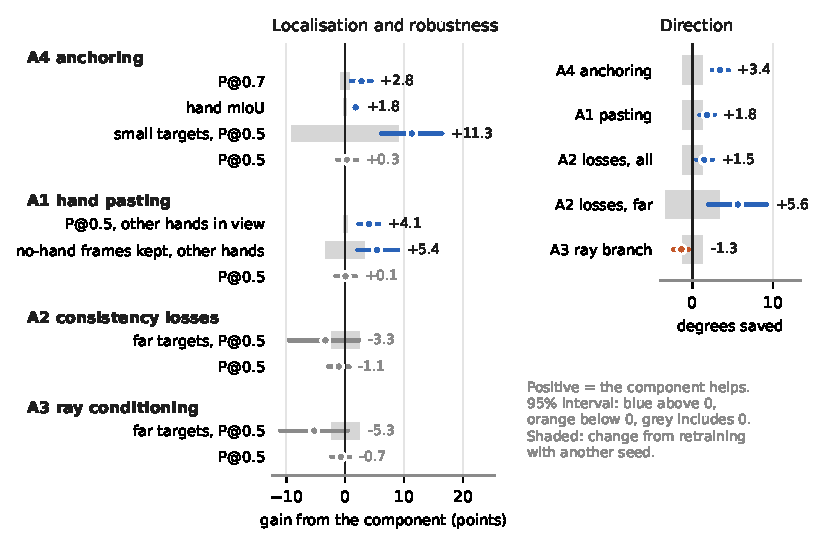
\includegraphics[width=\linewidth]{figures/ablation_effects}
  \caption{What each component contributes, with 95\% paired-bootstrap intervals. Gain = full model minus ablation, or degrees of direction error saved, so positive means the component helps. Grey bands: the largest change that retraining the full model with another seed produced on the same metric. ``Far'' in the labels denotes large-gap targets. The P@0.7 effect of A4 is not significant on the duplicate-free test split.}
  \Description{Interval plot with grey bands for retraining variation. Anchoring: P@0.7 +2.8, hand mIoU +1.8, small targets +11.3, all above zero and outside the bands; P@0.5 +0.3, crossing zero. Hand pasting: P@0.5 with other hands +4.1 and no-hand frames kept +5.4, above zero; P@0.5 +0.1. Consistency losses and ray conditioning: far-target and overall P@0.5 effects cross zero. Direction panel: degrees saved by anchoring 3.4, pasting 1.8, consistency losses 1.5 overall and 5.6 for far targets, all above zero; the ray branch -1.3, below zero.}
  \label{fig:ablation}
\end{figure}

\paragraph{A4, instance anchoring.} Against a plain model of the same size, the anchored chain improves hand mIoU by 1.8 points [+1.4, +2.2], against at most 0.3 between seeds, and lowers the direction error by 3.4$^\circ$ [2.4, 4.5], against at most 1.2$^\circ$. It also raises P@0.7 by 2.8 points [+1.1, +4.3] and small-target P@0.5 by 11.3 points [+6.5, +16.5] (the plain model's small boxes are drawn 2.4 instead of 1.9 times too large), but we treat these two as supporting evidence only: without duplicated test images the P@0.7 gain shrinks to 1.7 [0.0, +3.5], and the small-target gain is close to the seed spread (9.1). A4 also stopped earliest (best epoch 54, against 100), so its effects include a different training length.

\paragraph{A1, distractor pasting.} With other hands in view, the model trained with pasting keeps 4.1 more points of target P@0.5 [+2.4, +5.8] and 5.4 more points of no-hand frames as \emph{no hand} [+1.9, +8.9], and it puts its hand on another person's hand six times less often (0.2\% against 1.2\%). On clean images it costs nothing (P@0.5 $-$0.1) and even helps slightly (mIoU +1.2, hand mIoU +0.6, and 1.8$^\circ$ less direction error), which is consistent with pasting acting as a regulariser.

\paragraph{A2, consistency losses.} Without the two consistency terms, the direction error for large-gap targets rises by 5.6$^\circ$ [+2.1, +9.4], to 34.6$^\circ$, above all three seeds of the full model (29.0--32.3$^\circ$), and the overall direction error rises by 1.5$^\circ$, only slightly more than retraining alone changes it. Target-box accuracy does not change ($+$1.1 P@0.5, n.s.), because the target head does not draw on the predicted direction (A3). The losses therefore sharpen an output that an interface can use directly, for example to draw the pointing ray as feedback, but not the box.

\paragraph{Robustness of these conclusions.} Every difference reported above as an effect is significant under the paired bootstrap and larger than the change produced by retraining with another seed; effects close to that threshold (the small-target gain of anchoring, and the overall direction changes of A1--A3, 1.3--1.8$^\circ$ against 1.2$^\circ$) are supporting evidence only. Removing duplicated test images changes no conclusion except the P@0.7 effects of A3 and A4. The ablation variants stopped at different epochs (54 to 120), and some interventions are bundled (A1, A2 and A4).

\subsection{The Ray Prior and the Remedies We Tested}\label{app:ray}

\paragraph{What the ray branch learns.} Removing the ray branch $G^t$ (A3) changes P@0.5 by less than one point ($+$0.7, n.s.). P@0.7 rises by 1.9 points [+0.2, +3.6] and the direction error falls by 1.3$^\circ$, but the P@0.7 gain does not survive the duplicate check ($+$1.6 [$-$0.2, +3.3]), and A3 also trained 20\% longer (best epoch 120). Probing the trained full model shows why the branch adds nothing. The model does rely on it: its output is as large as the visual term (median ratio of spreads 0.86 on 500--800 test images), and switching it off at inference lowers P@0.5 on the whole test split from 58.9\% to 50.6\%. But it has learned proximity more than direction: its output correlates more with closeness to the fingertip ($\rho=-0.38$) than with closeness to the ray's line ($-0.27$), and on the probe subset hardly at all with being in front of the fingertip ($+0.04$). Accordingly, switching it off costs 11 points of P@0.5 on overlap targets and 9.5 on near ones in the probe subset, while on large-gap targets of the whole test split P@0.5 even rises by 2.0 points. A plausible reason is the training distribution: with 70\% overlap and 7\% large-gap targets, a ``near the fingertip'' prior already fits most targets, and the visual head can learn it by itself.

\paragraph{Remedies.} We retrained the 160\,px model three more times, each with one change and the seed and settings of the main run (Table~\ref{tab:remedies}). E1 lets the learned ray prior act only in front of the fingertip ($G^t$ is set to zero wherever $t_k<0$). E2 weights the target-box and target-heatmap losses three times as much for near and large-gap targets, the 30\% of training images in which the fingertip does not overlap the target. E3 spaces the $3\times3$ sample that predicts the target size two cells apart, so that it covers 40 instead of 24 pixels; none of the three adds a parameter. Neither remedy for large-gap targets works: E1 leaves P@0.5 unchanged and raises large-gap P@0.5 by 5.3 points with an interval that includes zero, while the direction error for large-gap targets grows by 4.3$^\circ$; E2 trades overlap accuracy ($-$3.8) and overall P@0.5 ($-$1.8) for near and large-gap gains that are not significant. A wider size sample (E3) does not tighten the boxes either (P@0.7 $-$1.2, small targets $+$1.3, both n.s.). Together with A2, A3 and the flat direction error across resolutions, these results locate the remaining bottleneck for large-gap targets in how the direction is estimated, not in how the ray prior is shaped or the training images are weighted. A direction supervised by the finger's own axis, for example from finger keypoints, remains untested.

\begin{table}[h]
  \caption{Remedies tested at 160\,px (one seed each; no extra parameters). Differences from the full model, in points (degrees for the direction error, where positive means worse); brackets: 95\% paired-bootstrap interval. Bold: the interval excludes 0 and the difference exceeds the largest change between the three seeds of the full model (P@0.5 0.1, P@0.7 0.8, overlap 0.5, large gap 2.4, small 9.1, hand mIoU 0.3, large-gap direction 3.4$^\circ$). Best epoch in parentheses (full model: 100).}
  \label{tab:remedies}
  \footnotesize
  \setlength{\tabcolsep}{2.5pt}
  \begin{tabular}{lrrrrrrr}
    \toprule
    Variant & P@0.5 & P@0.7 & Overlap & Large gap & Small & Hand mIoU & Dir.\ large gap ($^\circ$) \\
    \midrule
    Full model & 58.9 & 31.8 & 66.0 & 25.4 & 36.9 & 73.7 & 29.0 \\
    \midrule
    E1 forward-only ray prior (78) & $+$0.3 & $+$0.2 & $-$0.4 & $+$5.3 {\scriptsize[$-$0.5, +11.0]} & $-$4.2 & \textbf{$-$0.8} & \textbf{$+$4.3} \\
    E2 non-overlap targets $\times3$ (65) & \textbf{$-$1.8} & \textbf{$-$3.7} & \textbf{$-$3.8} & $+$3.8 {\scriptsize[$-$1.9, +9.6]} & $-$3.6 & \textbf{$-$1.2} & $-$0.8 \\
    E3 size sample spaced 2 cells (82) & $+$0.2 & $-$1.2 & $-$0.8 & $+$3.4 {\scriptsize[$-$2.4, +9.6]} & $+$1.3 & \textbf{$-$0.6} & \textbf{$+$3.7} \\
    \bottomrule
  \end{tabular}
\end{table}

\subsection{Backbone, IoU Curves and Examples}\label{app:backbone}

Table~\ref{tab:backbone} replaces the ShuffleNetV2 0.5$\times$ backbone with MobileNetV3-Small~\cite{howard2019mobilenetv3} or MobileNetV4-Conv-Small~\cite{qin2024mobilenetv4}, with the recipe otherwise unchanged. Neither changes P@0.5 significantly, while doubling or nearly tripling the parameters. Both lean towards better large-gap accuracy (intervals across 0) and a lower fingertip error (3.5 against 3.9\,px). Both runs stopped earlier (best epoch 64, against 100), so their numbers may be slightly low. Figure~\ref{fig:curves} shows how the share of successful hand and target boxes falls with the IoU threshold, and Figure~\ref{fig:qual} shows typical successes and one example of each failure type of Section~\ref{sec:failures}.

\begin{table}[h]
  \caption{Backbone swap at 160\,px, main-run recipe otherwise unchanged (one seed each). Target metrics in \%; brackets: 95\% paired-bootstrap interval of the difference from ShuffleNetV2.}
  \label{tab:backbone}
  \footnotesize
  \setlength{\tabcolsep}{4pt}
  \begin{tabular}{lrrrrrr}
    \toprule
    Backbone & Params & FP16 & GFLOPs & P@0.5 & Large-gap P@0.5 & Fingertip \\
    \midrule
    ShuffleNetV2 0.5$\times$ (ours) & 0.72M & 1.6\,MB & 0.231 & 58.9 & 25.4 & 3.9\,px \\
    MobileNetV3-Small & 1.57M & 3.2\,MB & 0.255 & 58.1 [$-$2.7, +1.0] & 31.1 [$-$0.5, +12.0] & 3.5\,px \\
    MobileNetV4-Conv-Small & 1.99M & 4.1\,MB & 0.398 & 59.8 [$-$0.9, +2.8] & 30.1 [$-$1.0, +10.5] & 3.5\,px \\
    \bottomrule
  \end{tabular}
\end{table}

\begin{figure}[h]
  \centering
  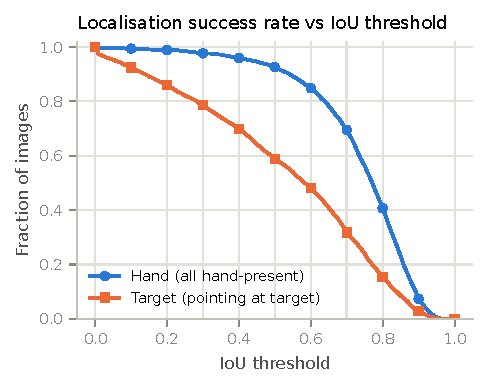
\includegraphics[width=0.48\linewidth]{figures/results/iou_success_rate}
  \caption{Share of test images whose hand or target box reaches each IoU threshold.}
  \Description{Two curves of success rate against IoU threshold; the hand curve stays above 0.9 up to IoU 0.5 and falls after 0.7, while the target curve falls steadily, reaching 0.59 at IoU 0.5 and 0.32 at 0.7.}
  \label{fig:curves}
\end{figure}

\begin{figure}[h]
  \centering
  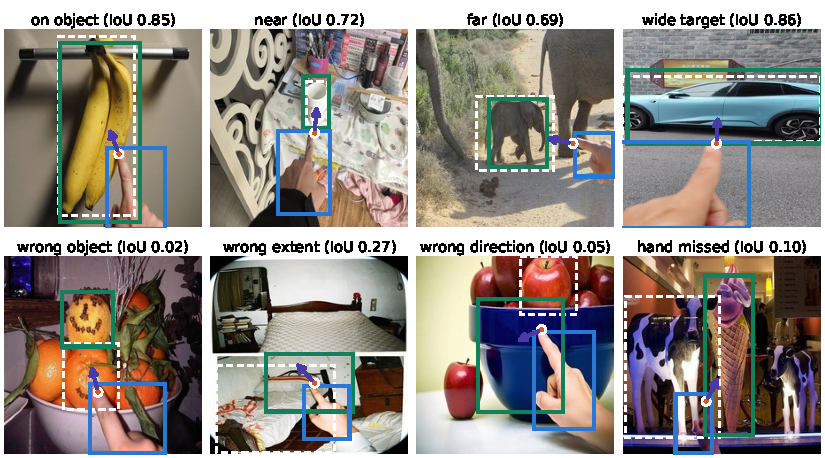
\includegraphics[width=\linewidth]{figures/qualitative}
  \caption{Successes (top) and failures (bottom) on EgoPoint test images: predicted hand (blue), fingertip and direction, and target (green); labelled target dashed. Bottom row, one example per failure type of Section~\ref{sec:failures}.}
  \Description{Eight egocentric images. Top row: correct target boxes for bananas touched by the finger, a cup near the finger, a young elephant far from the finger, and a car. Bottom row: a box on the wrong orange in a bowl of oranges, a box on part of a bed instead of the labelled bed, a box on a bowl while the label is an apple above it, and a frame where the hand gate missed the hand.}
  \label{fig:qual}
\end{figure}


\end{document}
